% !TeX root = presentation.tex
% !TeX program = xelatex
% ============================================================
%  Potential-Based Reward Shaping for Planar Pushing
%  Single-Agent Control vs Asymmetric Self-Play
%  Master Thesis Presentation — 30 minutes, 16:9
%  Theme: SimplePlusAIC (requires XeLaTeX or LuaLaTeX)
% ============================================================
\PassOptionsToPackage{table,dvipsnames}{xcolor}
\documentclass[aspectratio=169,xcolor=dvipsnames,t]{beamer}
\usepackage{fontspec}  % REQUIRED before theme for Epilogue font
\usepackage{colortbl}  % required for \rowcolor in tables
\usetheme{SimplePlusAIC}

\usepackage{amsmath,amssymb,amsfonts}
\usepackage{bm}
\usepackage{graphicx}
\usepackage{booktabs}
\usepackage{multirow}
\usepackage{tikz}
\usetikzlibrary{positioning,arrows.meta}
\usepackage{hyperref}

% --- Override AIC logo (not applicable to University of Groningen) ---
\logo{}

% --- Clean footline (institute removed; already on title slide; avoids \litfooter collisions) ---
\setbeamertemplate{footline}{%
  \begin{beamercolorbox}[ht=2em,sep=0.75em,wd=\paperwidth,leftskip=0.5cm,rightskip=0.5cm]{footlinecolor}
    \hfill
    \scriptsize{\insertframenumber}
  \end{beamercolorbox}%
}

% --- Custom colors (complementary to theme's Bordeaux/DarkBordeaux/Astronaut) ---
\definecolor{hlblue}{RGB}{0,102,204}
\definecolor{hlgreen}{RGB}{0,140,60}
\definecolor{hlred}{RGB}{190,30,30}
\definecolor{lightgray}{RGB}{220,220,220}

% --- Literature footer ---
\newcommand{\litfooter}[1]{%
  \vspace{2pt}%
  \hrule%
  \vspace{2pt}%
  {\tiny\color{LightDarkGrey} #1}%
}

% --- Full-bleed image frame (plain, no title/footer) ---
\newcommand{\fullbleedframe}[1]{%
  \begin{frame}[plain]
    \centering
    \includegraphics[width=\paperwidth,height=\paperheight,keepaspectratio]{#1}%
  \end{frame}%
}

% --- Media box: show image if present, else a labeled placeholder ---
% #1 = width fraction of \textwidth, #2 = file name in figures/
\newcommand{\mediabox}[2]{%
  \IfFileExists{figures/#2}{%
    \includegraphics[width=#1\textwidth]{figures/#2}%
  }{%
    \setlength{\fboxsep}{6pt}%
    \fcolorbox{LightDarkGrey}{lightgray}{%
      \begin{minipage}[c][0.26\textheight][c]{#1\textwidth}%
        \centering\small\itshape [clip placeholder]\\[3pt]
        \texttt{\footnotesize \detokenize{figures/#2}}\\[3pt]record \& drop file here%
      \end{minipage}%
    }%
  }%
}

% --- Clickable "play clip" link (works in Okular / Adobe via run:) ---
\newcommand{\playclip}[1]{\href{run:figures/#1}{\scriptsize\color{hlblue}$\blacktriangleright$ play clip}}

% --- Title info ---
\title[PBRS for Planar Pushing]{Potential-Based Reward Shaping \\for Planar Pushing}
\subtitle{Single-Agent Control vs.\ Asymmetric Self-Play}
\author{Vlad Iftime s3426394}
\institute[University of Groningen, FSE]{Faculty of Science and Engineering, Artificial Intelligence \\ University of Groningen}
\date{June 2026}

% --- Final page text ---
\finalpagetext{Thank You — Questions?}

\newcommand{\sectionframe}[1]{%
  \begin{frame}[plain]\centering\vfill
    {\color{hlblue}\Huge\textbf{#1}}\vfill\end{frame}}

\begin{document}

% ============================================================
% TITLE PAGE (theme macro)
% ============================================================
\addtobeamertemplate{title page}{\vspace{-14pt}}{}
\maketitlepage

% ~~~~~ SPEAKER NOTES ~~~~~
\note[itemize]{
\item 30-minute master thesis presentation
\item Topic: potential-based reward shaping for planar pushing with a UR5e robot arm
\item Five model variants: PPO-Baseline, PPO-PBRS, PPO-Curriculum, ASP-dPose, TASP-dPose
\item Key result: simplest model (PPO-PBRS, 80.0\%) beats every structured variant
\item Curriculum is competitive but adds no value; self-play degrades performance
}

% ============================================================
% SLIDE 0 — OVERVIEW
% ============================================================

\sectionframe{1.\ Introduction \& Research Questions}


\begin{frame}[t]{Outline}
  \footnotesize
  \begin{columns}[T,onlytextwidth]
    \begin{column}{0.48\textwidth}
      \begin{enumerate}
        \item \textbf{Introduction \& Research Questions}
        \item \textbf{Background \& Related Work} \\ {\scriptsize reward shaping · curriculum \& self-play · push mechanics \& SE(2)}
        \item \textbf{Problem Definition \& MDP}
        \item \textbf{Implementation} \\ {\scriptsize five models: PPO-Baseline, PPO-PBRS, PPO-Curriculum, ASP-dPose, TASP-dPose}
      \end{enumerate}
    \end{column}
    \begin{column}{0.48\textwidth}
      \begin{enumerate}
        \setcounter{enumi}{4}
        \item \textbf{Evaluation} \\ {\scriptsize 30 held-out scenes · 20 trials · Isaac vs gym}
        \item \textbf{Results}
        \item \textbf{Discussion}
        \item \textbf{Conclusion \& Takeaways}
      \end{enumerate}
    \end{column}
  \end{columns}
\end{frame}

% ~~~~~ SPEAKER NOTES ~~~~~
\note[itemize]{
\item Outline in eight parts, standard thesis structure
\item Background covers the five literature areas; Implementation describes all models; Evaluation defines the protocol; Results and Discussion present and interpret the validation outcomes
\item One-line thesis: PBRS single-agent wins; curriculum is competitive but adds no value; self-play degrades performance
}


\begin{frame}[t]{Research Questions}
  \begin{block}{Three Research Questions }
    \begin{enumerate}
      \item \textbf{RQ1:} Does asymmetric self-play match single-agent training in a contact-rich planar goal-reaching task under a single-GPU budget?
      \item \textbf{RQ2:} Which single dimension, among goal coupling, reward formulation, imitation signal, goal representation, and compute scale, accounts for the self-play outcome?
      \item \textbf{RQ3:} What mechanism prevents self-play from generalising its training-time success?
    \end{enumerate}
  \end{block}

  \vspace{2pt}
  \vfill\litfooter{[Sukhbaatar et al.\ 2018]~[Plappert et al.\ 2021]~\textbf{[Ng et al.\ 1999]}~[Narvekar et al.\ 2020]}
\end{frame}

% ~~~~~ SPEAKER NOTES ~~~~~
\note[itemize]{
\item RQ1: does asymmetric self-play match single-agent training in this contact-rich task under a single-GPU budget? Answer: no — single-agent solves 79--80\%, self-play transfers 0\%
\item RQ2: which of five dimensions (goal coupling, reward formulation, imitation signal, goal representation, compute scale) accounts for the self-play outcome? Answer: the coupled multi-objective gate
\item RQ3: what mechanism prevents self-play from generalising? Answer: training-time competence confined to Alice's own goal distribution, with a stale value function under the non-stationary distribution
\item Supporting RQ: does PBRS reach success with fewer environments than the improvement reward? (reward-efficiency comparison)
}


\sectionframe{2.\ Background \& Related Work}


\begin{frame}[t]{Reward Shaping (PBRS)}
  \textbf{Potential-based reward shaping} :
  \[ \mathcal{R}'(s,a,s') = \mathcal{R}(s,a,s') + \underbrace{\gamma\Phi(s')-\Phi(s)}_{F} \]
  \begin{itemize}
    \item \textbf{Policy invariance:} $Q'(s,a)=Q(s,a)-\Phi(s)$ — the optimal policy is unchanged for \emph{any} state potential $\Phi$.
    \item \textbf{Episodic validity} : $\gamma_{\text{shaping}}{=}1$ is safe — $\sum F=\Phi(s_T)-\Phi(s_0)$ is bounded.
    \item \textbf{Dynamic / arbitrary potentials}  — basis for our exponential $\Phi$.
  \end{itemize}
  \textbf{Why it matters here:} lets us design a dense, well-behaved reward \emph{without} changing the task's optimum — the foundation of every model in this thesis.
  \vfill\litfooter{[Ng et al.\ 1999]~\textbf{[Grze\'s 2017]}~[Devlin \& Kudenko 2012]~[Harutyunyan et al.\ 2015]}
\end{frame}

% ~~~~~ SPEAKER NOTES ~~~~~
\note[itemize]{
\item PBRS is the theoretical foundation — Ng et al.\ proved you can add $\gamma\Phi(s')-\Phi(s)$ to any reward without changing what the agent learns
\item Policy invariance: the optimal policy is unchanged — you can design rewards purely for learning speed
\item Episodic validity (Grzes 2017): $\gamma_{\text{shaping}}=1$ is safe in finite-horizon tasks — the shaping telescopes to $\Phi(s_T)-\Phi(s_0)$
\item Our exponential potentials $\Phi(s)=w e^{-k d^2}$ build on Devlin \& Kudenko's dynamic potential framework
\item This decoupling from policy is the core insight — reward engineering becomes a separate, principled task
}

\begin{frame}[t]{Curriculum \& Asymmetric Self-Play}
  \begin{columns}[T,onlytextwidth]
    \begin{column}{0.50\textwidth}
      \textbf{Forced curricula}
      \begin{itemize}
        \item \textbf{Surveys} 
        \item \textbf{Reverse / goal} : start near the goal, expand outward
        \item \textbf{Precision} : gradually tighten the success tolerance
      \end{itemize}
      \textbf{Our use:} a forced 3-phase pos$\to$rot curriculum (PPO-Curriculum)
    \end{column}
    \begin{column}{0.50\textwidth}
      \textbf{Automatic (self-play)}
      \begin{itemize}
        \item \textbf{ASP} : Alice/Bob adversarial game + ABC
        \item \textbf{Time-based Alice} : $R_A\propto t_B\!-\!t_A$, self-regulating
        \item \textbf{Regret-based} 
      \end{itemize}
      \textbf{Our use:} ASP-dPose (outcome) and TASP-dPose (time-based)
    \end{column}
  \end{columns}
  \vfill\litfooter{[Narvekar et al.\ 2020]~[Portelas et al.\ 2020]~\textbf{[Sukhbaatar et al.\ 2018]}~[Plappert et al.\ 2021]}
\end{frame}

% ~~~~~ SPEAKER NOTES ~~~~~
\note[itemize]{
\item Forced curricula: Narvekar and Portelas surveys show curriculum helps when rewards are sparse or exploration is hard
\item Our PPO-Curriculum uses a 3-phase pos$\to$rot staging — position first, then progressively add rotation
\item Automatic curricula (self-play): ASP (Sukhbaatar, Plappert) trains Alice and Bob adversarially — Alice proposes goals, Bob solves them
\item Time-based Alice (Sukhbaatar 2018): $R_A \propto t_B - t_A$ creates a self-regulating curriculum where Alice is rewarded for finding goals Bob struggles with
\item Regret-based methods (PAIRED, AMIGo): antagonist minimizes protagonist's regret — solvable but challenging environments
\item Our use: we test both outcome-based (ASP-dPose) and time-based (TASP-dPose) variants
}

\begin{frame}[t]{Geometry \& Mechanics of Planar Pushing}
  \begin{columns}[T,onlytextwidth]
    \begin{column}{0.62\textwidth}
      \textbf{Push mechanics}
      \begin{itemize}
        \item \textbf{Quasi-static pushing}: motion set by the friction limit surface.
        \item \textbf{Limit-surface normality}: \emph{every} push couples translation and rotation.
      \end{itemize}

      \vspace{4pt}
      \textbf{SE(2) geometry}
      \begin{itemize}
        \item \textbf{Unified distance}: a single scalar that combines position and orientation error, weighted by the object's physical size $L$
        \item \textbf{Equivariant manipulation}: exploiting SE(2)/SO(2) symmetry.
      \end{itemize}

      \vspace{4pt}
      \textbf{Our use:} the SE(2) $d_{\text{pose}}$ provides a unified reward for the self-play variants.
    \end{column}
    \begin{column}{0.36\textwidth}
      \vspace{6pt}
      \centering
\includegraphics[width=\textwidth]{figures/diagram_limit_surface.png}
    \end{column}
  \end{columns}


  \vfill\litfooter{[Mason 1986]~[Goyal et al.\ 1991]~[Park 1995]~[Urain et al.\ 2023]}
\end{frame}

% ~~~~~ SPEAKER NOTES ~~~~~
\note[itemize]{
\item Quasi-static pushing (Mason 1986): the object motion is slow enough that inertial forces are negligible — the limit surface fully determines behavior
\item Limit-surface normality (Goyal 1991): the resulting motion twist $\mathbf{t}$ is always normal to the limit surface — every push couples translation AND rotation
\item SE(2) Lie-group distance (Park 1995): fuses position and orientation error into a single geodesic metric with characteristic length $L$
\item Equivariant manipulation: exploiting SO(2) rotational symmetry so learned pushing skills transfer across orientations
\item Why this matters: limit-surface coupling explains why the combined pos+rot gate is the universal bottleneck across all our models
}

\sectionframe{3.\ Problem Definition \& MDP}


\begin{frame}[t]{Planar-Pushing MDP — State, Action \& Transition}
  \begin{columns}[T]
    \begin{column}{0.58\textwidth}
      \textbf{State} $\mathbf{s} \in \mathbb{R}^{28}$: EE pose (6) $|$ object pose (14) $|$ goal pose (6) $|$ errors (2)

      \vspace{4pt}
      \textbf{Action} $\mathbf{a} \in \mathbb{R}^4$ (object-relative): $(r,\phi,\ell,\theta)$ — 21 bins/dim, 194\,481 discrete actions

      \vspace{6pt}
      \textbf{Transition} : $\mathbf{t}\propto\nabla f(\mathbf{w})$ — limit-surface normality couples \textbf{every} push with rotation

      \vspace{4pt}
      \textbf{Success:} pos $<$ 5\,cm \textbf{and} rot $<$ 0.2\,rad.  \textbf{Validation:} 30 scenes $\times$ 20 trials $\times$ up to 30 pushes
    \end{column}
    \begin{column}{0.38\textwidth}
      \centering
      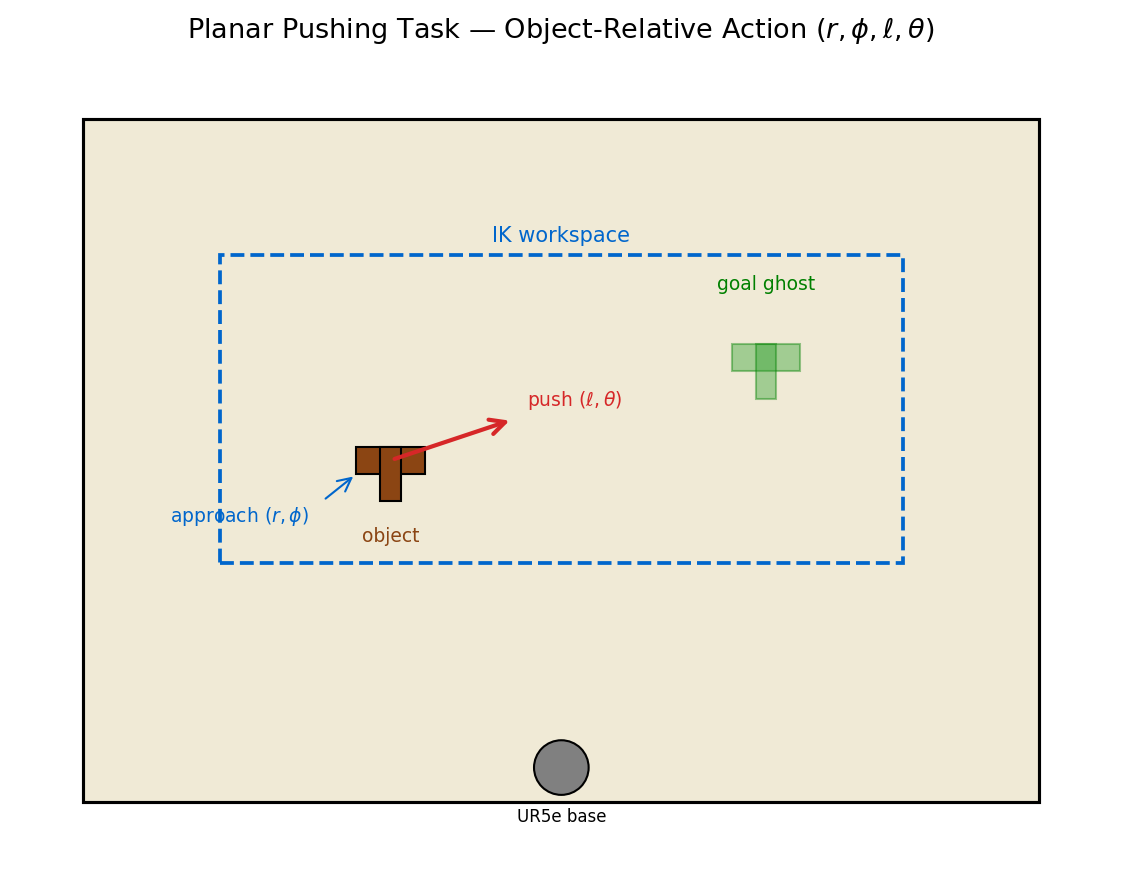
\includegraphics[width=0.95\textwidth]{figures/diagram_task_schematic.png}
    \end{column}
  \end{columns}

  \vfill\litfooter{[Mason 1986]~[Lynch \& Mason 1996]~[Goyal et al.\ 1991]}
\end{frame}

\note[itemize]{
\item Planar pushing MDP: UR5e robot pushes a T-block on a 1.4m×1.0m table. 28D obs, 4D object-relative macro-action (21 bins/dim = 194k discrete). Object-relative actions achieve ~95\,\% contact rate.
\item Transition: limit-surface normality couples translation and rotation — every push does both.
\item Success: pos < 5\,cm AND rot < 0.2\,rad. Validation: 30 held-out scenes × 20 trials × up to 30 pushes/trial; scene solved if any trial meets the gate.
}



\begin{frame}[t]{How the Fractional Reward Failed}
  \textbf{Fractional improvement formula:}\\
  $R = \underbrace{\textcolor{hlblue}{\alpha\!\cdot\!\frac{d_{\text{prev}}-d_{\text{now}}}{d_{\text{prev}}}}}_{\text{improvement}}
       - \underbrace{\textcolor{Orange}{\beta_{\text{pos}}\!\cdot\!d_{\text{now}}}}_{\text{pos penalty}}
       - \underbrace{\textcolor{hlred}{\beta_{\text{rot}}\!\cdot\!y_{\text{now}}}}_{\text{rot penalty}},\quad
       \alpha{=}3.0,\;\beta_{\text{pos}}{=}0.5,\;\beta_{\text{rot}}{=}0.25$

  \vspace{4pt}
  \textbf{Worked example} — pushing toward a goal 30\,cm away, 1\,cm improvement:
  \[
  R = \textcolor{hlblue}{3.0\!\cdot\!0.01/0.30}
     - \textcolor{Orange}{0.5\!\cdot\!0.29}
     - \textcolor{hlred}{0.25\!\cdot\!0.5}
     = \textcolor{hlred}{\mathbf{-0.17}}
  \]

  \vspace{4pt}
  \begin{columns}[T]
    \begin{column}{0.50\textwidth}
      {\footnotesize \textbf{Problem 1 — Negative reward for progress:} the
penalty terms dominate the improvement.}
    \end{column}
    \begin{column}{0.46\textwidth}
      {\footnotesize \textbf{Problem 2 — Near-zero variance:} 99\% of pushes produce $R \in [-0.5,+0.1]$. }
    \end{column}
  \end{columns}

  \vfill\litfooter{[Ng et al.\ 1999]~[Grzes \& Kudenko 2009]~[Schulman et al.\ 2017]}
\end{frame}

% ~~~~~ SPEAKER NOTES ~~~~~
\note[itemize]{
\item The fractional formula gives $\sim$0 or negative reward for 99\% of pushes. A 1\,cm improvement from 30\,cm earns $-0.17$ — negative reward for genuine progress
\item The penalty terms $\beta d_{\text{now}}$ and $\beta_{\text{rot}} y_{\text{now}}$ dominate the fractional improvement term $\alpha \Delta d / d_{\text{prev}}$, making the net reward negative even for progress-producing pushes
\item PPO multiplies the policy gradient by the advantage sign. Negative advantage → gradient pushes policy AWAY from goal-directed behavior
\item Sparse bonuses (+5/+2) fire on only $\sim$1\% of pushes. At 528 envs × 15 pushes = 7,920 steps/iter, that's $\sim$79 bonus events — too few to overcome the noise
}


\begin{frame}[t]{How PBRS Fixes the Reward}
  \textbf{PBRS potential:} $\Phi(s) = w\!\cdot\!e^{-k\cdot d^2},\quad k{=}30,\;w{=}10$

  \vspace{4pt}
  \textbf{Same push, same 1\,cm improvement:}
  \[
  R = \textcolor{hlblue}{w\!\cdot\!\big[e^{-k\cdot d_{\text{now}}^2} - e^{-k\cdot d_{\text{prev}}^2}\big]}
     = \textcolor{hlblue}{10\!\cdot\!\big[e^{-30\cdot0.29^2} - e^{-30\cdot0.30^2}\big]}
     = \textcolor{hlgreen}{\mathbf{+0.133}}
  \]

  \vspace{4pt}
  \textbf{Why this matters:}
  \begin{itemize}
    \item \textbf{Correctly signed} — every push toward the goal gets positive reward, away gets negative
    \item \textbf{Bounded} — $\Phi(s) \in [0,w]$, so $|R| \le w$ regardless of distance or physics glitches
    \item \textbf{Markovian} — depends only on current state $s$, not on history or $d_{\text{prev}}$
    \item \textbf{Policy-invariant} — the optimal policy under PBRS is identical to the original task
  \end{itemize}

  \vfill\litfooter{[Ng et al.\ 1999]~[Grze\'s 2017]~[Harutyunyan et al.\ 2015]}
\end{frame}

% ~~~~~ SPEAKER NOTES ~~~~~
\note[itemize]{
\item PBRS replaces the fractional formula with $\Phi(s')-\Phi(s)$ — a state-only potential difference that is always correctly signed
\item The same push earns $+0.133$ with PBRS vs $-0.17$ with the old formula. The sign reversal is the key — gradient now pushes TOWARD the goal
\item Four properties make PBRS ideal: bounded (no reward explosions from physics glitches), Markovian (GAE-compatible), correctly signed (every push provides useful signal), policy-invariant (optimal policy unchanged per Ng et al.)
\item PBRS provides a guaranteed signal floor on every push regardless of distance — the agent always knows which direction is "better"
}


\sectionframe{4.\ Implementation}


\begin{frame}[t]{Why Isaac Lab?}
  \begin{columns}[T,onlytextwidth]
    \begin{column}{0.48\textwidth}
      \footnotesize
      \begin{enumerate}
        \item \textbf{GPU-batched parallelism} — 528 simultaneous environments produce 7{,}920-sample PPO batches. gym-pusht peaks at 960 — 8$\times$ smaller. Large batches stabilize the non-stationary self-play gradient.
        \item \textbf{No extra per-iteration cost} — self-play and single-agent run at identical wall-clock ($\sim$0.022\,it/s). The two-agent machinery adds negligible overhead.
      \end{enumerate}
    \end{column}
    \begin{column}{0.50\textwidth}
      \centering
      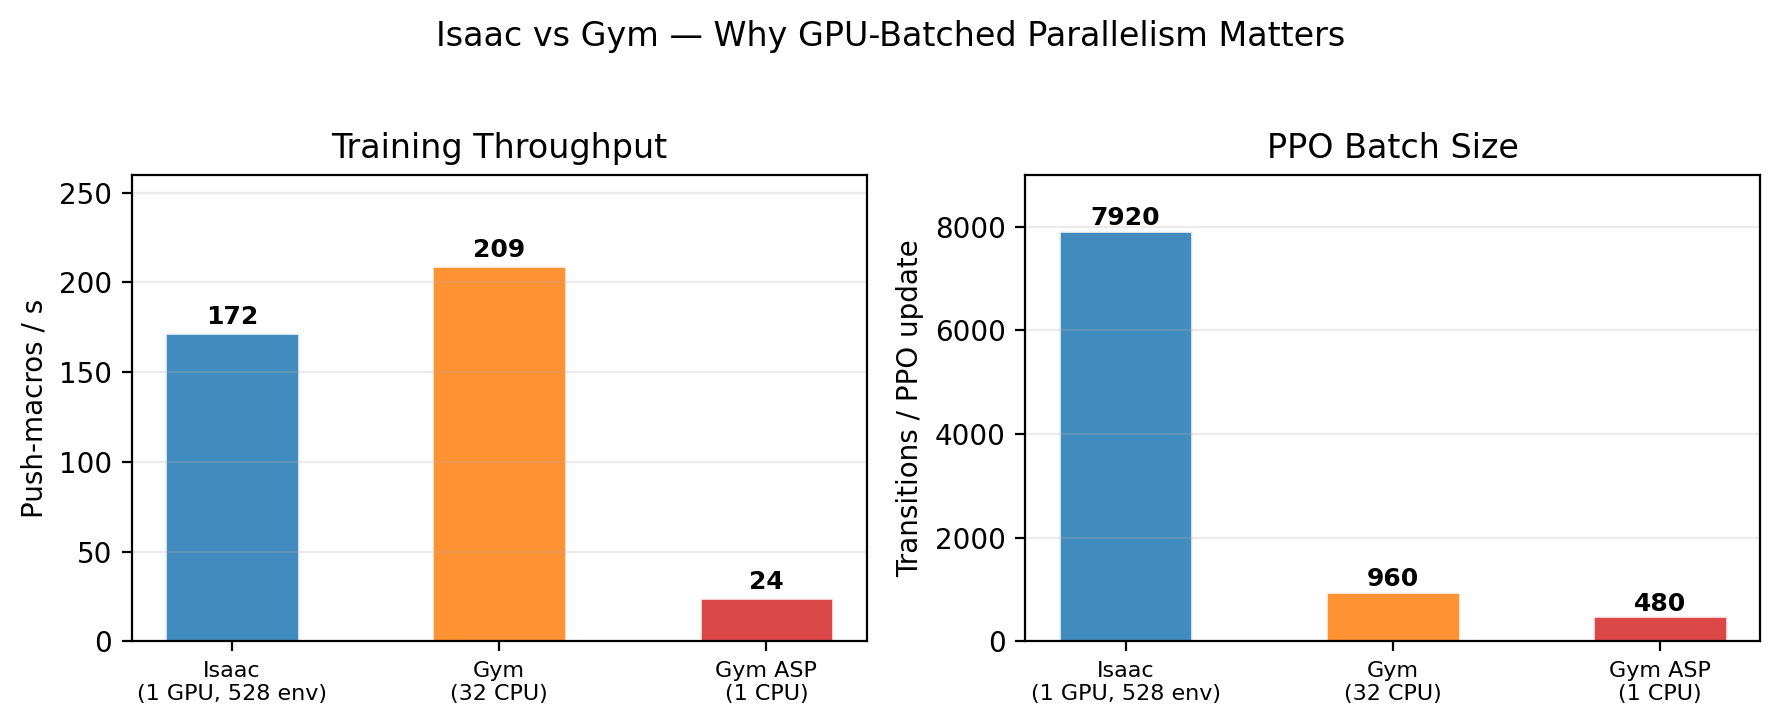
\includegraphics[width=\textwidth,height=0.55\textheight,keepaspectratio]{figures/isaac_vs_gym.png}
      \vspace{2pt}
      {\footnotesize Throughput is comparable; batch size is the differentiator.}
    \end{column}
  \end{columns}
\end{frame}

\begin{frame}[t]{Why Isaac Lab? - Training demos}
  \begin{columns}[T,onlytextwidth]
 
  \end{columns}
\end{frame}

% ~~~~~ SPEAKER NOTES ~~~~~
\note[itemize]{
\item Isaac GPU-batched: 528 envs stepped in parallel → 7{,}920 transitions per PPO update. gym-pusht HPC at 32 CPU cores only reaches 960 per update. Large batches are essential to stabilize PPO+LSTM gradients under non-stationary self-play objectives
\item Throughput (isaac\_vs\_gym.png): Isaac 172 push/s at 528 envs vs Gym 209 push/s at 32 cores — raw speed is comparable. The 8× batch-size difference drives the performance gap, not raw throughput
\item Self-play and single-agent run at identical per-iteration wall-clock (\textasciitilde0.022 it/s) on the same GPU — the 2-agent machinery (Alice + Bob, GoalEncoder, ABC) adds no measurable overhead
\item Takeaway: Isaac gives self-play its best shot — same budget, same batch size as the winning single-agent — and it still reaches only 6.7--16.7\% SR. The 4.8× gap is structural, not a compute artifact
}

\begin{frame}[t]{Results — Single-Agent Baselines vs Self-Play}
  \textbf{Same PPO+LSTM, same push primitive, same 528-env budget, 5 seeds:}
  \vspace{4pt}
  \begin{center}
  \begin{tabular}{lccc}
    \toprule
    \textbf{Model} & \textbf{Scene SR} & \textbf{Pos-only} & \textbf{Pos+rot} \\
    \midrule
    \rowcolor{hlgreen!15}
    PPO-PBRS & \textcolor{hlgreen}{\textbf{79.3\%}} & 100\% & 69\% \\
    \rowcolor{hlgreen!15}
    PPO-Curriculum & \textcolor{hlgreen}{\textbf{80.0\%}} & 100\% & 70\% \\
    ASP-dPose (outcome) & \textcolor{hlred}{\textbf{0.0\%}} & 0\% & 0\% \\
    TASP-dPose (time) & \textcolor{hlred}{\textbf{0.0\%}} & 0\% & 0\% \\
    ASP-disc (position-only) & 7.3\% & --- & --- \\
    \bottomrule
  \end{tabular}
  \end{center}

  \vspace{4pt}
  {\small \text{\emph{Single-agent baselines solve $\sim$4 in 5 scenes; self-play transfers none.}  \textcolor{hlred}{\textbf{Self-play's training-time success never reaches held-out scenes.}}}}
  {\scriptsize \textit{(5 seeds; ASP-disc validated on its own position-only disc scenes.)}}

  \vfill\litfooter{[Ng et al.\ 1999]~[Narvekar et al.\ 2020]~\textbf{[Sukhbaatar et al.\ 2018]}~[Plappert et al.\ 2021]}
\end{frame}

% ~~~~~ SPEAKER NOTES ~~~~~
\note[itemize]{
\item The two single-agent baselines — plain PBRS (79.3\%) and PBRS with a forced curriculum (80.0\%) — both solve roughly four in five held-out scenes; the curriculum adds nothing on top of the already well-shaped reward
\item Both solve every position-only scene (100\%) and only fail on rotation-requiring scenes (69--70\%) — position is never the problem
\item The self-play subjects transfer nothing: ASP-dPose and TASP-dPose are at 0.0\% in every seed, under both Alice reward formulations
\item ASP-disc — the same self-play loop on a rotationally symmetric disc with a position-only goal — retains only 7.3\%, isolating the coupled gate as the factor that removes self-play's residual generalisation
\item Training-time rates tell the opposite story (ASP-dPose logs 35.8\% per-push), so the failure is a generalisation gap, not a lack of learning
}


\begin{frame}[t]{All Models at a Glance}
  \centering\small
  \begin{tabular}{lll}
    \toprule
    \textbf{Model} & \textbf{Idea} & \textbf{Reward / curriculum} \\
    \midrule
    \textbf{PPO-Baseline} & single agent, original reward & fractional improvement (non-PBRS) \\
    \rowcolor{hlgreen!15}
    \textbf{PPO-PBRS} & single agent, no curriculum & two-potential PBRS (pos, rot) \\
    \textbf{PPO-Curriculum} & single agent + staged curriculum & PBRS + forced pos$\to$rot \\
    \textbf{ASP-dPose} & self-play (Alice/Bob) & SE(2) PBRS, outcome Alice ($+5/-1$) \\
    \textbf{TASP-dPose} & self-play (Alice/Bob) & SE(2) PBRS, time-based Alice \\
    \bottomrule
  \end{tabular}

  \vspace{6pt}
  {\small All five models share the same PPO+LSTM backbone and object-relative push primitive.}
  \vfill\litfooter{[Schulman et al.\ 2017]~[Ng et al.\ 1999]~\textbf{[Sukhbaatar et al.\ 2018]}}
\end{frame}

\begin{frame}[t]{PPO-PBRS — Single-Agent (Recommended Baseline)}
  \small
  \textbf{Architecture:} Single PPO agent, LSTM(28$\to$256) + MLP[512, 256] trunk, MultiCategorical head (4 dims $\times$ 21 bins). No curriculum, no Alice/Bob, no GoalEncoder.

  \textbf{Training:} 528 envs, 15 pushes/rollout, $\sim$3000 iterations $\sim$1.6 days wall-clock ($\sim$0.022 it/s).

  \textbf{Why it works:}
  \begin{enumerate}
    \item \textbf{Dense, bounded gradient} — PBRS fires on every push
    \item \textbf{Fixed goal distribution} — stationary random goals; no adversarial shift
    \item \textbf{Single network} — one agent, one optimizer; no multi-agent instability
  \end{enumerate}

  \vfill\litfooter{[Ng et al.\ 1999]~[Grze\'s 2017]~[Schulman et al.\ 2017]}
\end{frame}

% ~~~~~ SPEAKER NOTES ~~~~~
\note[itemize]{
\item PPO-PBRS is the simplest possible architecture: single PPO agent with LSTM+MLP, PBRS reward, sparse completion bonuses
\item Three reasons it works: PBRS provides dense gradient at every push, fixed random goal distribution avoids adversarial shift, single network avoids multi-agent optimization instability
\item Converges within 1500 iterations. Stable value function bounded by exponential potentials
}


\begin{frame}[t]{PBRS vs Fractional— Reward Signal Analysis}
  \begin{columns}[T,onlytextwidth]
    \begin{column}{0.48\textwidth}
      \centering
      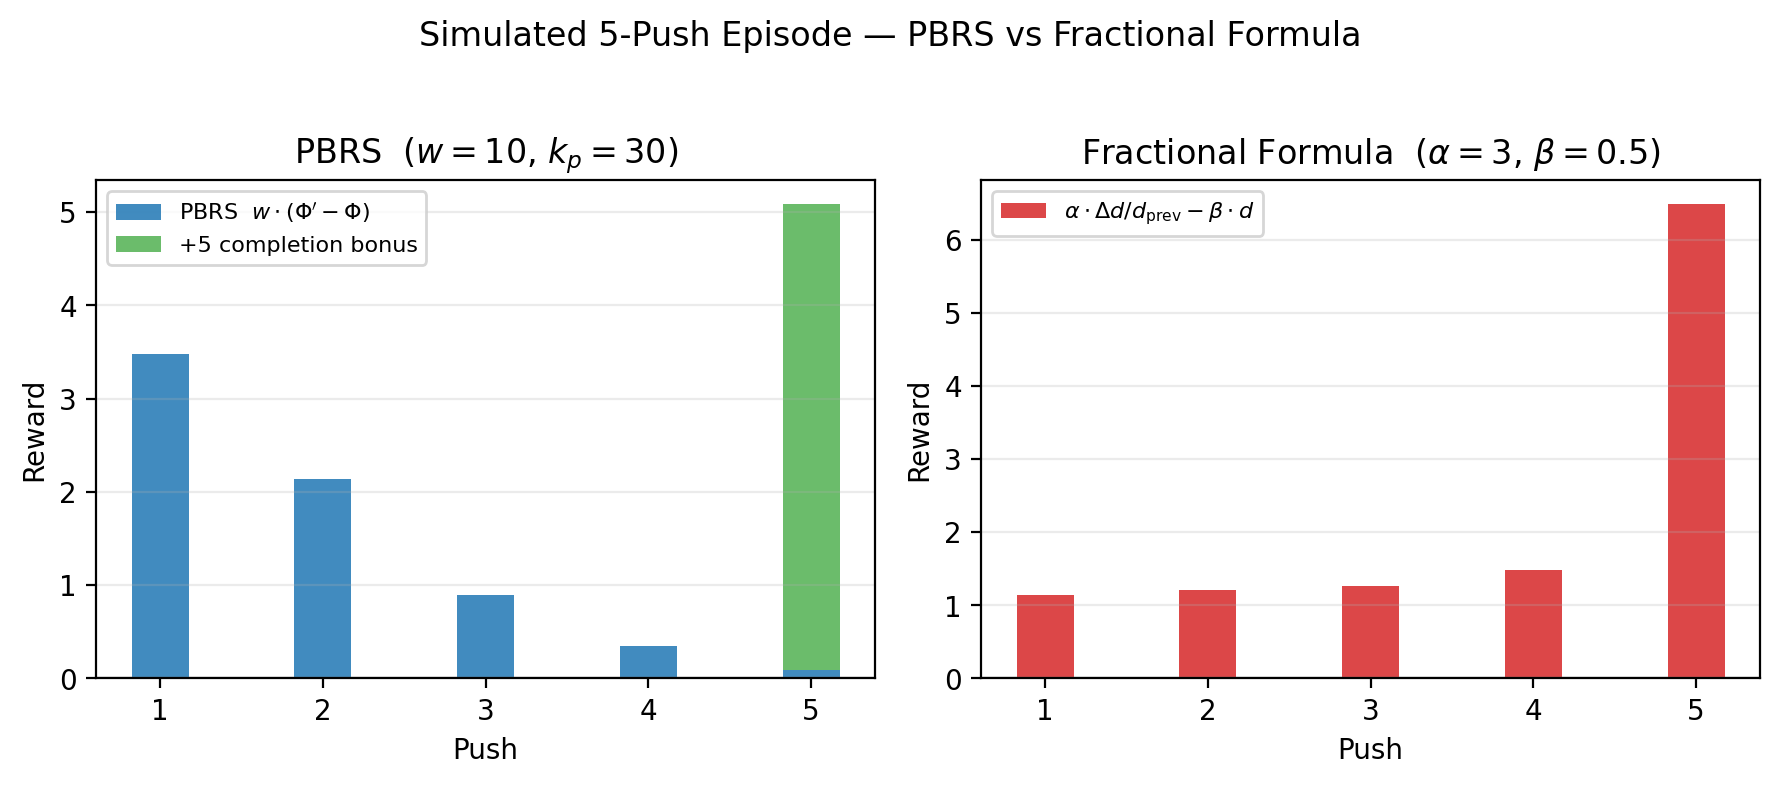
\includegraphics[width=1.0\textwidth]{figures/a3_episode_simulation.png}
      \vspace{2pt}
      {\footnotesize\textbf{Per-push reward — Fractional vs PBRS:} same 5-push episode. Fractional formula: negative or zero for 80\% of pushes. PBRS: correctly-signed, bounded on every push.}
    \end{column}
    \begin{column}{0.48\textwidth}
      \centering
      
\includegraphics[width=1.0\textwidth]{figures/a5_Position_Error.png}
      \vspace{2pt}
      {\footnotesize\textbf{Position error per iteration (TensorBoard):} PBRS at 528 envs converges to lower PosErr than fractional formula at 2{,}048 envs — 4$\times$ more environment-efficient.}
    \end{column}
  \end{columns}

  \vspace{4pt}
  \begin{center}
  \small Dense signal on every push, bounded rewards, stable value — PBRS avoids the gradient starvation and critic instability of the old fractional formula.
  \end{center} 

\end{frame}

% ~~~~~ SPEAKER NOTES ~~~~~
\note[itemize]{
\item Left: simulated 5-push episode comparing PBRS vs fractional formula per-push reward. PBRS gives correctly-signed positive reward on every push; fractional formula gives negative or near-zero reward
\item Right: actual TensorBoard data from training runs — PBRS at 528 envs converges to lower position error (~0.095 m) than the fractional formula at 2,048 envs (~0.150 m) despite 4× fewer parallel environments
\item Both achieve 80\% validation SR — PBRS does it with 4× fewer envs. The fractional formula works at scale but needs more parallelism to overcome its gradient starvation
}


\begin{frame}[t]{Why PBRS for ASP? — Decoupling Advantage from Value}
  \textbf{GAE advantage decomposes into two parts:}
  \[
  \hat{A}_t = \underbrace{\sum (\gamma\lambda)^l\,
  \big[\textcolor{hlblue}{\Phi(s_{t+l+1}) - \Phi(s_{t+l})}\big]}_{\textcolor{hlblue}{\text{always correctly-signed}}}
  \;+\; \underbrace{\sum (\gamma\lambda)^l\,
  \big[\gamma V(s_{t+l+1}) - V(s_{t+l})\big]}_{\textcolor{hlred}{\text{biased when $V$ is stale}}}
  \]

  \vspace{6pt}
  \begin{columns}[T]
    \begin{column}{0.48\textwidth}
      \textbf{\textcolor{hlblue}{$\Phi$-term:} PBRS potential difference}\\
      {\small $\Phi(s) = w\!\cdot\!e^{-k\cdot d^2}$ increases when object moves toward goal. Correct sign on every push regardless of $V(s)$ accuracy.}
    \end{column}
    \begin{column}{0.48\textwidth}
      \textbf{\textcolor{hlred}{$V$-term:} value function bootstrap}\\
      {\small Under ASP, Alice shifts goal distribution $\rightarrow$ $V(s)$ perpetually stale. GAE bootstraps from wrong values $\rightarrow$ biased advantage.}
    \end{column}
  \end{columns}

  \vspace{6pt}
  \begin{center}
  \textbf{Outcome:} \textcolor{hlblue}{PBRS lifts ASP 0\% $\to$ 16.7\%} via the $\Phi$-term —\\
  but only partially, because the \textcolor{hlred}{$V$-term bias remains}.\\
  \textcolor{hlgreen}{Single-agent: no distribution shift $\to$ $V$ accurate $\to$ both align $\to$ 80\%.}
  \end{center}

\end{frame}

% ~~~~~ SPEAKER NOTES ~~~~~
\note[itemize]{
\item GAE normally sums TD errors $\delta_t = r_t + \gamma V(s_{t+1}) - V(s_t)$. Under ASP with sparse rewards, those errors are just V-noise
\item PBRS adds $\Phi(s')-\Phi(s)$ to every step — this term is always correct because $\Phi$ increases when object moves toward goal
\item The $\Phi$-term provides a floor of correctly-signed gradient signal even when Bob's $V(s)$ is completely wrong
\item This is why PBRS lifts ASP from 0\% to 16.7\% — Bob gets genuine learning signal despite the non-stationary objective
\item But it only partially rescues ASP because the $V$-component still contributes bias. Single-agent has no distribution shift → $V$ is accurate → both terms align → 80\%
}


\begin{frame}[t]{SE(2) Unified Distance — Self-Play Variants}
  \begin{columns}[T,onlytextwidth]
    \begin{column}{0.54\textwidth}
      \textbf{SE(2) metric:} $d_{\text{pose}} = \sqrt{dx^2 + dy^2 + L^2 d\theta^2}$
      \begin{itemize}
        \item Single scalar combining $(dx,dy)$ and $d\theta$; $L$ = char.\ length (T-block $0.07$\,m)
        \item \textbf{Single-potential PBRS:} $\Phi(s)=w\,e^{-k\,d_{\text{pose}}^2}$, $k=30,\,w=10$
        \item Eliminates competing pos/rot gradients — aligns reward with the coupled physics
      \end{itemize}
      \textbf{Result:} SE(2) does \emph{not} rescue self-play — ASP-dPose reaches only 6.7\% validation SR vs single-agent 80\%. The self-play curriculum is the root cause, not the metric.
    \end{column}
    \begin{column}{0.44\textwidth}
      \centering
      
\includegraphics[width=1.0\textwidth]{figures/diagram_limit_surface.png}
    \end{column}
  \end{columns}

  \vfill\litfooter{[Park 1995]~[Urain et al.\ 2023]~[Lynch \& Mason 1996]}
\end{frame}

% ~~~~~ SPEAKER NOTES ~~~~~
\note[itemize]{
\item The SE(2) unified distance replaces separate position and rotation errors with a single Riemannian metric on the planar rigid-body configuration space
\item L converts radians to meters. For the T-block with L=0.07m, 0.5 rad of rotation contributes 3.5cm to d_pose — roughly equal weight with a 3.5cm position displacement
\item The single-potential PBRS eliminates the competing gradient problem: separate pos/rot potentials each pull in different directions, while the SE(2) potential provides a unified gradient
\item Both ASP-dPose (SE(2) self-play) collapses just like the separate-potential self-play — the SE(2) metric doesn't rescue the self-play dynamics, confirming the curriculum is the root cause, not the reward metric
}


% \begin{frame}[t]{TASP-dPose-BobPenalty — The Fallout}
%   \textbf{Added to TASP-dPose:} Bob time penalty $R_B \mathrel{+}= -\gamma_{sp}\!\cdot\!t_B$  on \emph{all} phase ends.

%   \vspace{4pt}
%   \textbf{Valid SR: \textcolor{hlred}{0.0\%}} (0/30 scenes, 2600 iters, 528 envs) — worse than no-penalty TASP-dPose (16.7\%).

%   \vspace{4pt}
%   \textbf{Mechanism — the penalty fires on catastrophes (tip/launch/OOB):}
%   \begin{center}\small
%   \begin{tabular}{lccc}
%     \toprule
%     \textbf{Trajectory} & \textbf{PBRS Dense + Sparse} & \textbf{Penalty ($0.5\times t_B$)} & \textbf{Total} \\
%     \midrule
%     Fail on push 1  & $-10.5$ & $-0.5$ & $\mathbf{-11.0}$ \\
%     Fail on push 10 & $-15.0$ & $-5.0$ & $\mathbf{-20.0}$ \\
%     Succeed push 5  & $+10.0$ & $-2.5$ & $\mathbf{+7.5}$ \\
%     \bottomrule
%   \end{tabular}
%   \end{center}

%   {\small PPO gradient pushes Bob toward ``fail on push 1'' ($-11.0$ beats $-20.0$). Alice's reward collapses: $R_A = 0.5\!\cdot\!\max(0,1-5) = 0$. \textbf{The symmetric reward creates a perverse fail-fast equilibrium.} Asymmetric (Alice incentivised, Bob unpenalised) is necessary.}
%   {\scriptsize \textit{(See Appendix I for full mechanism breakdown.)}}

%   \vfill\litfooter{[Sukhbaatar et al.\ 2018]~[Letcher et al.\ 2019]~[Plappert et al.\ 2021]}
% \end{frame}

% % ~~~~~ SPEAKER NOTES ~~~~~
% \note[itemize]{
% \item Model I (TASP-dPose-BobPenalty) trains the full symmetric Sukhbaatar reward: Alice time bonus + Bob time penalty
% \item Result: 0\% SR — worse than no-penalty TASP-dPose at 16.7\%. The penalty fires on ALL phase ends including catastrophes
% \item Bob learns that failing on push 1 ($-$11.0) is a better return than trying for 10 pushes and failing ($-$20.0). PPO's gradient pushes toward faster failure
% \item Alice gets zero reward ($t_B \approx 1$ gives $R_A = 0$) — the self-regulating curriculum collapses on both sides
% \item This is NOT an indictment of Sukhbaatar 2018 or Letcher 2019. It's a reward design failure: the penalty applied to catastrophe environments creates a degenerate equilibrium
% \item Lesson: asymmetric reward structure (Alice incentivised, Bob unpenalised) is necessary in this domain
% }


\begin{frame}[t]{PPO-Curriculum — Position$\to$Rotation Curriculum }
  \textbf{Design:} Same PPO agent as PPO-PBRS + 3-phase curriculum:
  \begin{enumerate}
    \item $w_{\text{rot}}=0$, position-only training
    \item Triggered when episodic position-SR $\ge 0.5$ for 20 iters: $w_{\text{rot}}$ ramps $0\to10$ over 200 iters
    \item Full PBRS (multi-objective)
  \end{enumerate}


  \vspace{2pt}
  \textbf{Trigger:} gates on episodic position-only SR $\ge$ 0.5 over a 20-iter lookback. Curriculum now activates and reaches \textcolor{hlgreen}{76.7\% SR} — only 3.3pp below PPO-PBRS.
  

  \vfill\litfooter{[Narvekar et al.\ 2020]~[Portelas et al.\ 2020]~[Florensa et al.\ 2017]}
\end{frame}

% ~~~~~ SPEAKER NOTES ~~~~~
\note[itemize]{
\item P82 trigger fix: old gate used per-push mean PosErr < 0.08m AND over 50 iterations — unreachable. Best model's per-push mean PosErr plateaus at {\textasciitilde}0.10m, never below 0.08m. Fix: episodic position-only SR ≥ 0.5 over 20 iterations.
\item Corrected PPO-Curriculum achieves 76.7\% SR, 3.3pp below PPO-PBRS. Curriculum works; doesn't beat the simpler no-curriculum baseline.
\item Position precision improves from Phase 1 training (0.023m vs 0.032m); rotation slightly worse (0.663 vs 0.568 rad).
}


\begin{frame}[t]{ASP Loop — Alice$\leftrightarrow$Bob Cycle}
  \centering
  \vspace{-4pt}

  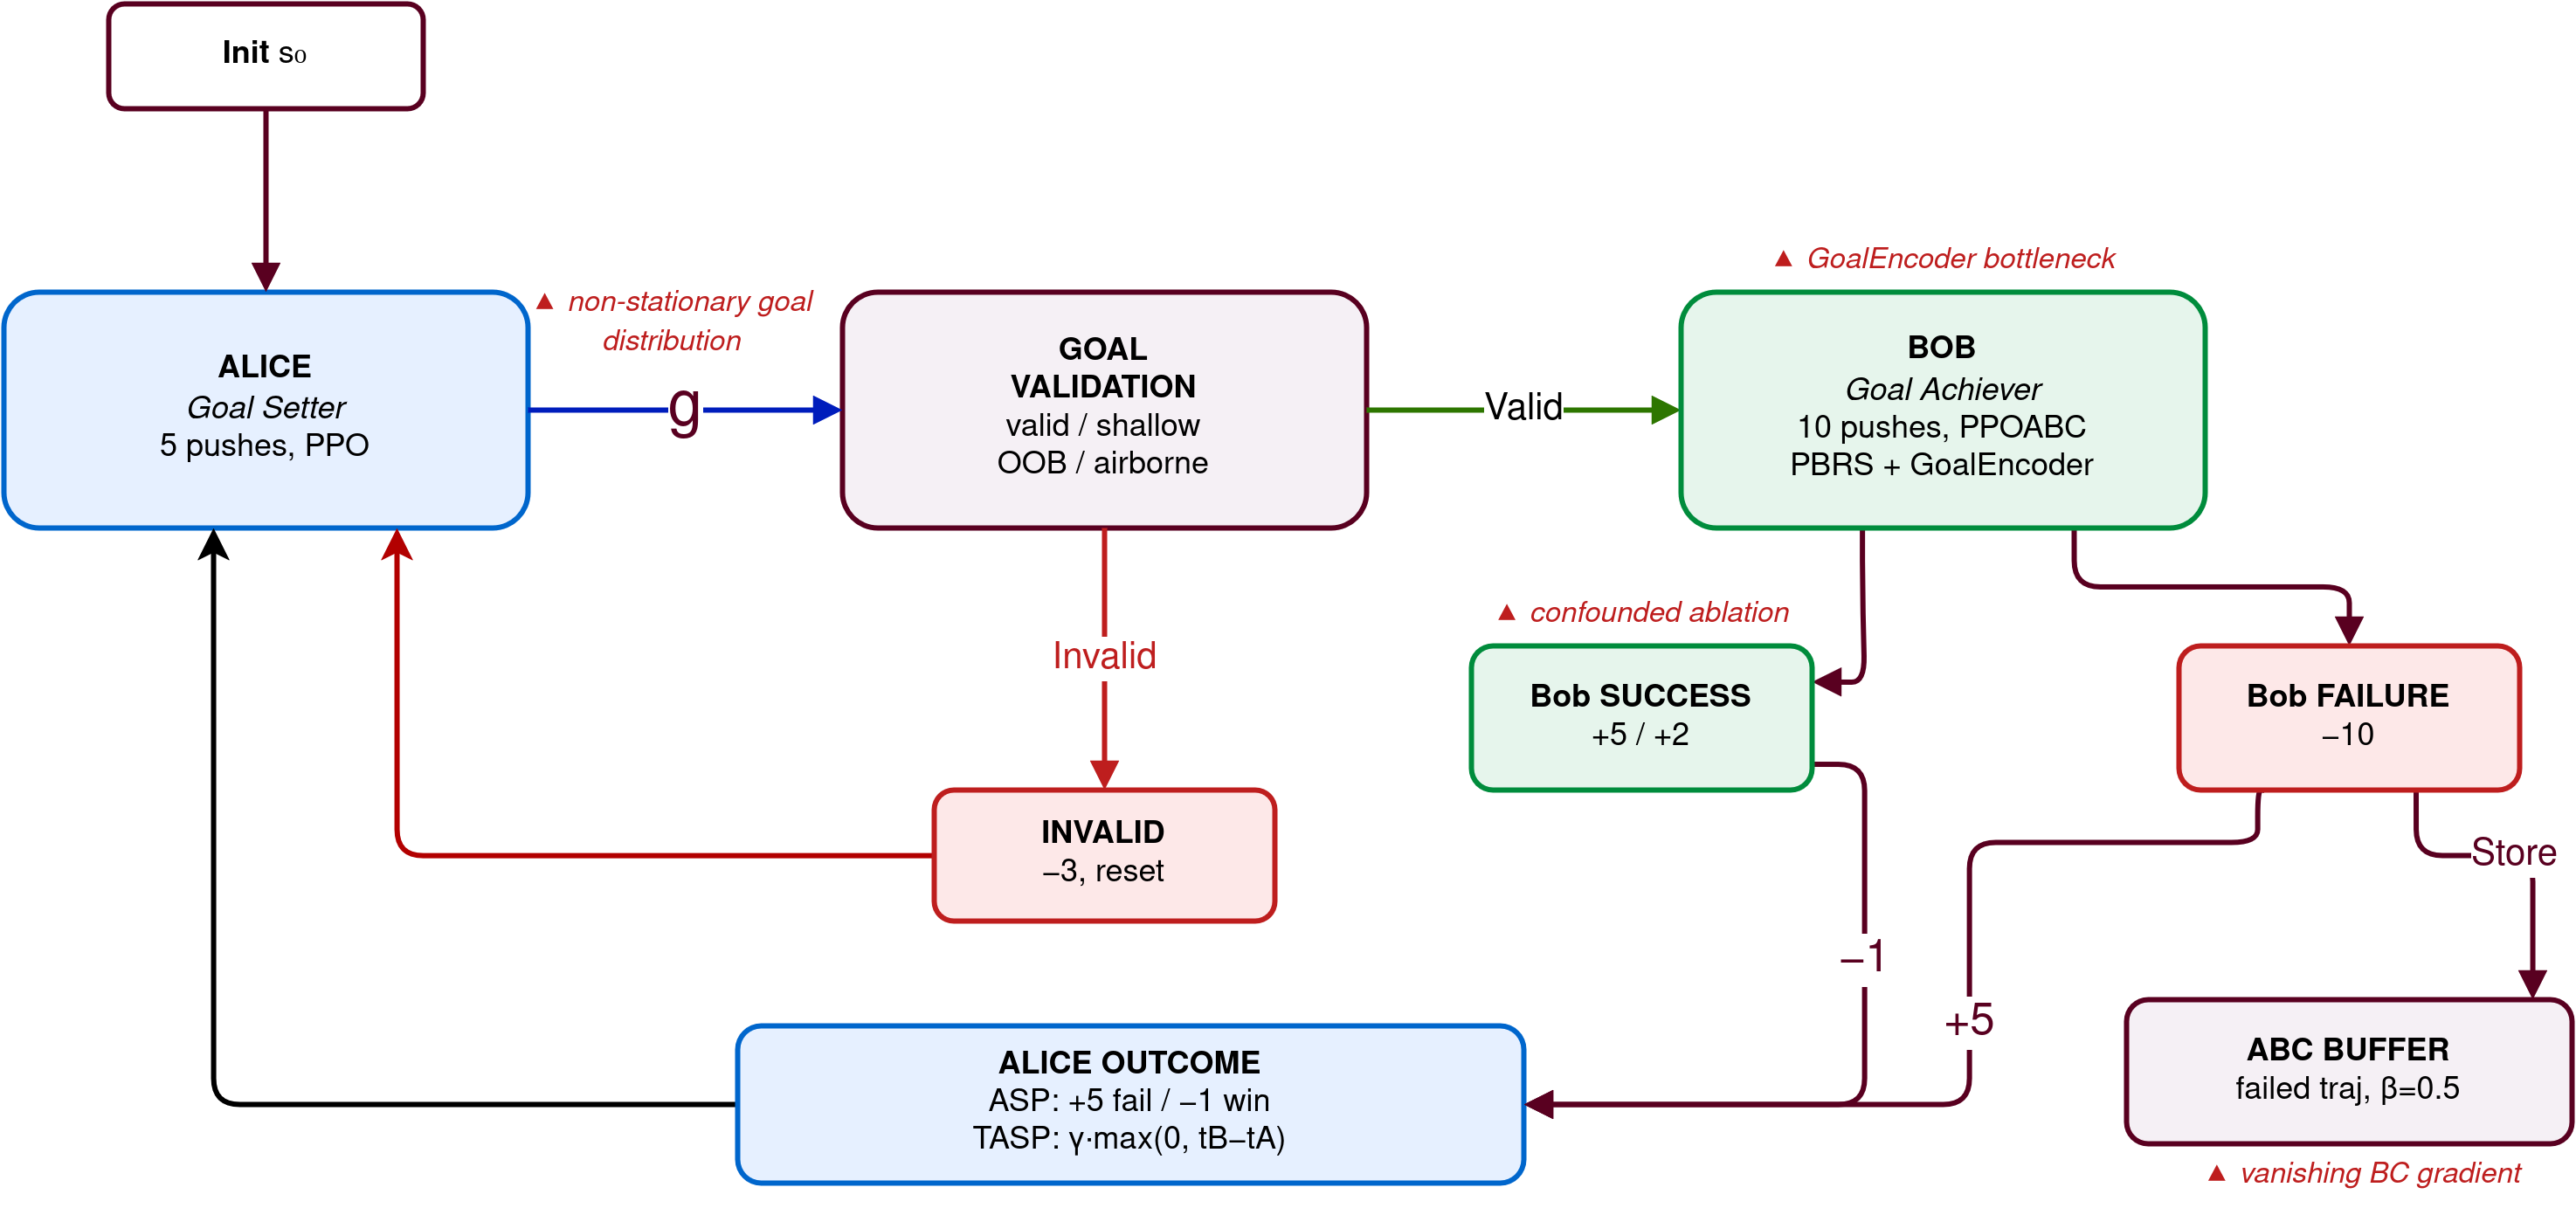
\includegraphics[width=\textwidth,height=0.85\textheight,keepaspectratio]{figures/asp_loop_diagram.png}

\end{frame}

% ~~~~~ SPEAKER NOTES (ASP loop + failure mode detail) ~~~~~
\note[itemize]{
\item Alice: 5-push free-roaming phase, object-relative $(r,\phi,\ell,\theta)$ actions, no goal observation, PPO agent. Final object pose $g$ passed to goal validation.
\item Goal validation: valid ($>\!0.10$\,m displacement, $+1$), shallow ($-1$), OOB/airborne ($-3$), too-easy ($-3$, reset). Invalid goals reset the episode; valid goals proceed to Bob.
\item Bob: starts from a clean reset at $s_0$; 10 pushes with PBRS dense shaping + sparse completion bonuses ($+5$/$+2$). PPOABC + GoalEncoder $\phi{:}\mathbb{R}^{22}{\to}\mathbb{R}^{8}$ + LSTM. Success gate: $d_{\text{pose}}\!<\!0.055$\,m (SE2) or pos$<\!0.05$\,m \& rot$<\!0.2$\,rad. Failure: OOB/launched/tipped/max pushes ($-10$).
\item \textbf{Non-stationary goal distribution:} Alice learns continuously, so Bob's training distribution shifts every iteration. PPO importance ratio computed from rollouts collected under a previous Alice — dominated by distribution drift, not Bob's weight updates. (See Slides 9--9b.)
\item \textbf{GoalEncoder bottleneck:} $\phi{:}\mathbb{R}^{22}{\to}\mathbb{R}^{8}$ compresses object+goal into single 8D latent. Fine translation/yaw signal may be lost, preventing precise SE(2) alignment.
\item \textbf{Vanishing BC gradient:} Failed trajectories enter ABC buffer for BC ($\beta{=}0.5$). If Bob rarely succeeds, buffer fills with near-random trajectories — BC signal becomes noise.
\item \textbf{Confounded ablation:} Self-play vs single-agent differ on $\ge 7$ axes: agent count, goal distribution, episode budget, GoalEncoder, ABC, historical pool, update frequency. 4.8$\times$ SR gap cannot be attributed to any single lever (see the Caveat — Confounded Ablation slide).
}


\begin{frame}[t]{ASP-dPose vs TASP-dPose — Alice Reward}
  \textbf{Both share the SE(2) $d_{\text{pose}}$ Bob reward and T-block object; only Alice's reward differs.}

  \vspace{4pt}
  \begin{center}
  \small
  \begin{tabular}{lcc}
    \toprule
    \textbf{Self-play variant} & \textbf{Alice reward} & \textbf{Valid SR} \\
    \midrule
    \textbf{ASP-dPose} (outcome-based) & $R_A=+5$ fail $/-1$ win, $\beta_{\text{abc}}{=}0.5$ & \textcolor{hlred}{6.7\%} \\
    \textbf{TASP-dPose} (time-based) & $R_A=\gamma_{sp}\!\cdot\!\max(0,t_B\!-\!t_A)$, $\beta_{\text{abc}}{=}0.5$ & \textcolor{hlred}{16.7\%} \\
    \bottomrule
  \end{tabular}
  \end{center}

  % \vspace{4pt}
  % \textbf{Findings:}
  % \begin{itemize}
  %   \item Time-based Alice (TASP-dPose) outperforms outcome-based (ASP-dPose) by $+$10pp — both share ABC ($\beta{=}0.5$)
  %   \item Best self-play variant (TASP-dPose, 16.7\%) still \textbf{4.8$\times$} below single-agent (PPO-PBRS, 80.0\%)
  % \end{itemize}

  \vspace{2pt}
  {\scriptsize \textbf{Why ABC provides negligible gradient:} Bob's MultiCategorical policy (4\,dim $\times$ 21\,bins = 194\,K discrete actions) concentrates probability on goal-relevant pushes. Alice's unguided actions lie outside this concentration $\rightarrow$ $\pi/\pi_{\text{old}}$ ratio extreme $\rightarrow$ PPO clip activates $\rightarrow$ zero BC gradient despite $\beta{=}0.5$. Combined with non-repeatable push transitions, ABC contributes nothing.}

  \vfill\litfooter{[Plappert et al.\ 2021]~\textbf{[Sukhbaatar et al.\ 2018]}~[Dennis et al.\ 2020]}
\end{frame}

% ~~~~~ SPEAKER NOTES ~~~~~
\note[itemize]{
\item The two self-play variants differ only in Alice's reward: outcome-based (ASP-dPose) vs time-based (TASP-dPose), both with the SE(2) d\_pose Bob reward on the T-block
\item Time-based Alice intentionally aligns Alice's reward with solvable goals — she gains when Bob takes more pushes than she did
\item Time-based reward outperforms outcome-based: TASP-dPose 16.7\% vs ASP-dPose 6.7\%
\item But even the best self-play variant (TASP-dPose, 16.7\%) is 4.8× below single-agent PPO-PBRS (80.0\%)
\item ABC is present in both variants but provides negligible gradient: Plappert 2021's PPO-style BC loss clips $\pi/\pi_{\text{old}}$ — when Alice's random push demonstrations are too different from Bob's goal-directed policy, the ratio is extreme, the clip activates, and BC contributes zero gradient
\item In Plappert 2021's block grasping, Alice trajectories are smooth and repeatable. In our contact-rich planar pushing, every push couples translation and rotation (limit-surface normality), making Alice's trajectories poor, non-repeatable demonstrations. The PPO clipping mechanism designed to prevent aggressive BC updates inadvertently blocks all BC signal when the demonstration domain differs this much from the policy domain
}

\sectionframe{5.\ Evaluation}


\begin{frame}[t]{Validation Test Suite — Top 10 Held-Out Scenes}
  \centering
  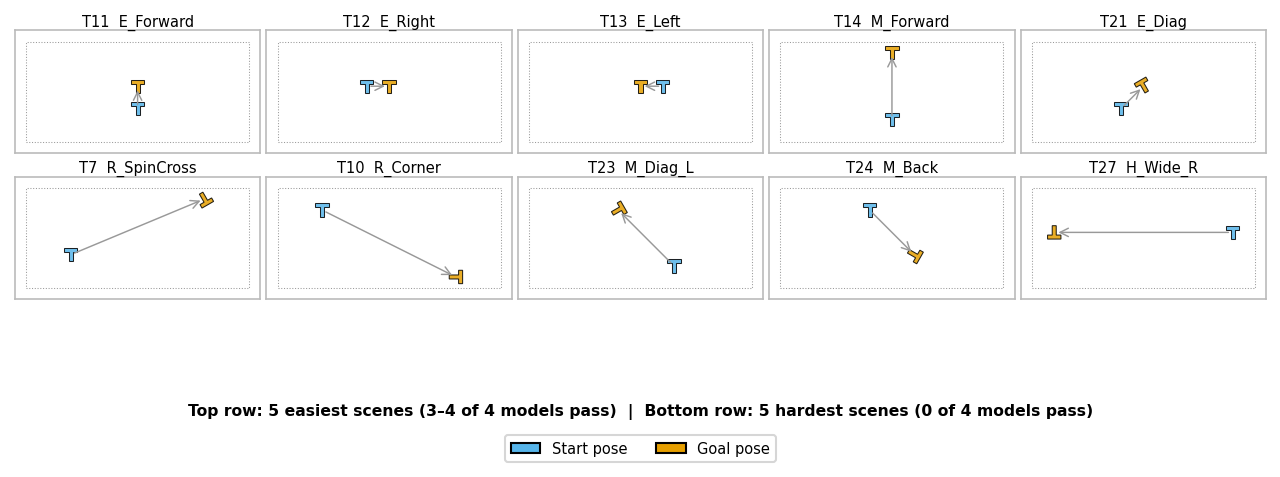
\includegraphics[width=\textwidth,height=0.80\textheight,keepaspectratio]{figures/val_test_layout_top10.png}

  \vspace{2pt}
  {\scriptsize T-block \textcolor[HTML]{56B4E9}{\textbf{start pose}} $\to$ \textcolor[HTML]{E69F00}{\textbf{goal pose}}. Every model is evaluated on an identical 30-scene suite (20 trials $\times$ up to 30 pushes per scene).}

\end{frame}

% ~~~~~ SPEAKER NOTES ~~~~~
\note[itemize]{
\item The full validation suite — 30 held-out T-block scenes, identical for every model
\item Row 1: rotation-dominant scenes (large yaw change); Row 2: position-only (goal yaw = 0); Row 3: combined position + rotation
\item Sky-blue = object start pose, orange = goal pose, arrow = required translation
\item Difficulty within each row spans easy/medium/hard by start-to-goal distance and yaw change
}

\begin{frame}[t]{What Does Success Look Like?}
  \begin{columns}[T,onlytextwidth]
    \begin{column}{0.30\textwidth}
      \centering
      \textbf{Position-only success}\\[4pt]
      
\includegraphics[width=0.9\linewidth]{figures/pos_succ.png}
    \end{column}
    \begin{column}{0.30\textwidth}
      \centering
      \textbf{Position + Rotation success}\\[4pt]
      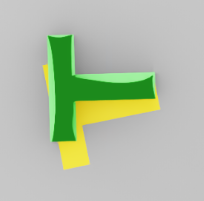
\includegraphics[width=0.9\linewidth]{figures/posrot_succ_pos_00-3_rot_0-17.png}
    \end{column}
    \begin{column}{0.38\textwidth}
      \vspace{4pt}
      {\small \textbf{Success gate:}}
      \begin{itemize}
        \item \textcolor{hlblue}{Object} reaches \textcolor{hlgreen}{goal} \\
              \textbf{pos $<$ 0.05\,m AND rot $<$ 0.2\,rad}
        \item 10/30 scenes are pos-only (rotation ungated)
        \item 20/30 scenes require both
        \item $\geq$1 of 20 trials must pass per scene
      \end{itemize}
    \end{column}
  \end{columns}
\end{frame}

% Push Mechanics detail moved to Related Work and Appendix A
% ============================================================
% ============================================================





\sectionframe{6.\ Results}


\begin{frame}[t]{Multi-Model Validation}
  \centering
  
\includegraphics[width=\textwidth,height=0.72\textheight,keepaspectratio]{figures/val_multi_combined.png}


\end{frame}

% ~~~~~ SPEAKER NOTES ~~~~~
\note[itemize]{
\item Dual-panel validation summary: left = overall SR bars with ±1 SE error bars, right = pos-only vs pos+rot breakdown
\item PPO-PBRS and PPO-Curriculum at 80.0\% and 76.7\% — overlapping error bars, 3.3pp gap not statistically significant (p>0.05, SE diff=±10.6pp)
\item Self-play variants clustered at 0--16.7\%, 4.8--11.9× below single-agent
\item Pos+rot is the universal bottleneck: single-agent 65--70\%, self-play 0--10\%
\item Single seed per model (training variance across 5 chains exists but validation is single-budget)
}


\begin{frame}[t]{PPO-PBRS — Validation Results}
  \begin{columns}[T,onlytextwidth]
    \begin{column}{0.50\textwidth}
      \textbf{30 held-out T-block scenes (20 trials each):}
      \begin{itemize}
        \item \textcolor{hlgreen}{\textbf{80.0\% SR}} (24/30) — pos-only \textbf{100\%}, pos+rot \textbf{70\%}
        \item PosErr \textbf{0.032\,m}, RotErr \textbf{0.568\,rad} (mean over all 30 scenes, incl.\ failures)
        \item Per-attempt (trial-level) SR \textbf{66\%}; scene SR counts a scene solved if any of its 20 trials passes
      \end{itemize}
    \end{column}
    \begin{column}{0.48\textwidth}
    \end{column}
  \end{columns}

  \vfill\litfooter{[Ng et al.\ 1999]~[Grze\'s 2017]~[Schulman et al.\ 2017]}
\end{frame}

% ~~~~~ SPEAKER NOTES ~~~~~
\note[itemize]{
\item Validation: 30 held-out T-block scenes, 20 trials per scene. 80.0\% scene SR
\item Perfect on position-only scenes (100\%), strong on combined pos+rot scenes (70\%)
\item PosErr 0.032m and RotErr 0.568 rad are averaged over all 30 scenes, including failures (RotErr is inflated by failed and by pos-only scenes whose rotation is ungated). On successful scenes PosErr $\approx$ 0.010m
\item Per-attempt SR is 66\% (396/600 trials); the 80\% scene SR counts a scene solved if any of its 20 trials passes
\item The overhead clip shows the trained PPO-PBRS policy recorded top-down
}


\begin{frame}[t]{PPO-PBRS — Per-Test Error}
  \centering
  \vspace{-2pt}
  \includegraphics[width=0.95\textwidth]{figures/pbrs_errors.png}\\[2pt]
  {\scriptsize 79.3\% $\pm$ 3.5\% (5 seeds) — 100\% pos-only, 69\% pos+rot. All failures are rotation-limited; position stays within tolerance on every scene. \textit{(one representative seed shown)}}

\end{frame}

\begin{frame}[t]{PPO-Curriculum — Per-Test Error}
  \centering
  \vspace{-2pt}
  \includegraphics[width=0.95\textwidth]{figures/curr_errors.png}\\[2pt]
  {\scriptsize 80.0\% $\pm$ 4.1\% (5 seeds) — 100\% pos-only, 70\% pos+rot. Equivalent to PBRS: the forced curriculum adds nothing once the reward is well shaped. \textit{(one representative seed shown)}}

\end{frame}

\begin{frame}[t]{TASP-dPose — Per-Test Error}
  \centering
  \vspace{-2pt}
  \includegraphics[width=0.95\textwidth]{figures/tasp_errors.png}\\[2pt]
  {\scriptsize 0.0\% (4 seeds) — no held-out scene solved; rotation never learned (RotErr $\sim$1.35\,rad). Training-time success does not transfer. \textit{(one representative seed shown)}}

\end{frame}

\begin{frame}[t]{ASP-dPose — Per-Test Error}
  \centering
  \vspace{-2pt}
  \includegraphics[width=0.95\textwidth]{figures/asp_errors.png}\\[2pt]
  {\scriptsize 0.0\% (5 seeds) — no held-out scene solved; rotation never learned (RotErr $\sim$1.44\,rad). Outcome-based Alice transfers nothing. \textit{(one representative seed shown)}}

\end{frame}

\begin{frame}[t]{ASP vs TASP training}
  \centering
  \vspace{-2pt}
  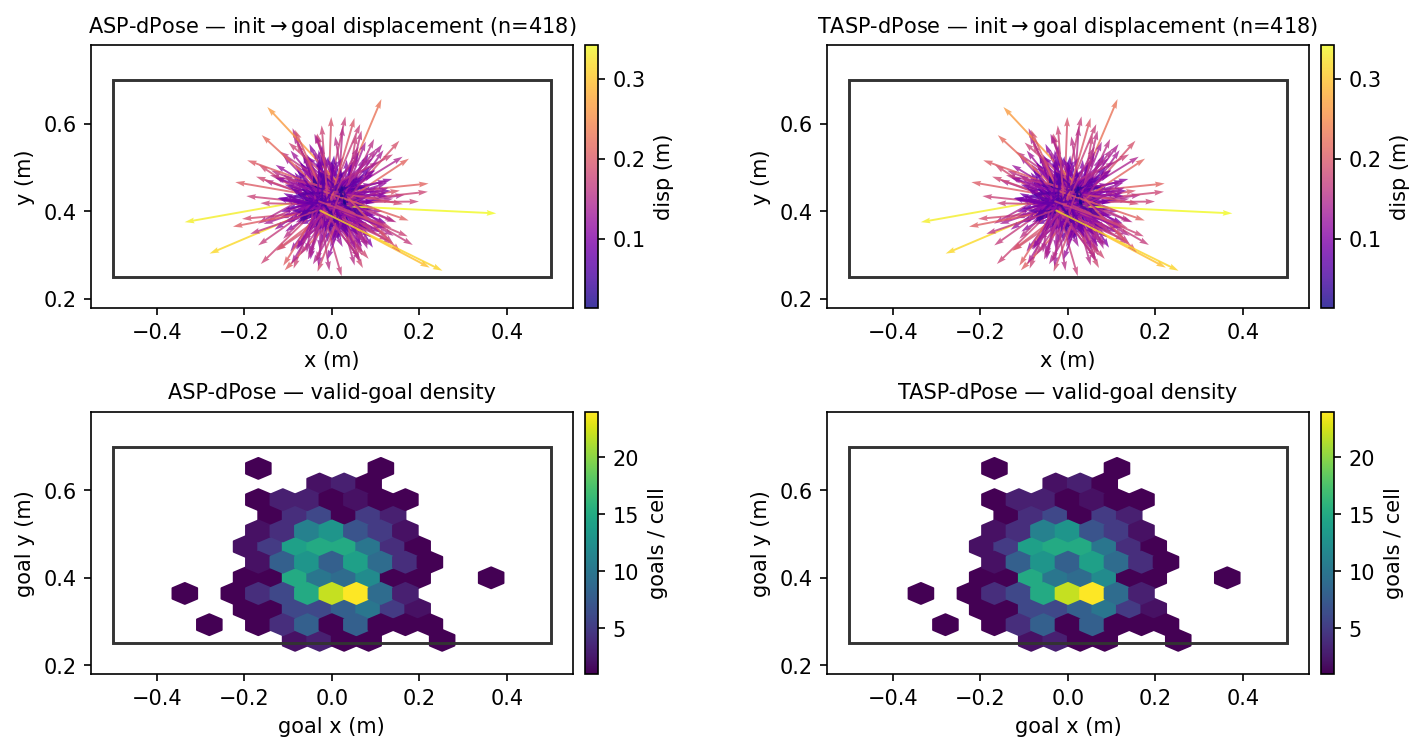
\includegraphics[width=\textwidth,height=0.62\textheight,keepaspectratio]{figures/asp_vs_tasp_training.png}\\[1pt]
  {\scriptsize ASP-dPose (outcome) vs TASP-dPose (time): goal displacement (top) and valid-goal density (bottom).}

\end{frame}

\begin{frame}[t]{PPO-PBRS — Validation Runs (overhead)}
  {\small Three held-out T-block scenes, top-down camera — the trained PPO-PBRS policy:}

 

\end{frame}

% ~~~~~ SPEAKER NOTES ~~~~~
\note[itemize]{
    {\small Self-play fails on \emph{both} axes across almost all scenes — rotation error stays $>$ 1.4 rad. The few successes are easy position-only scenes.}
    {\small Both clear position on nearly every scene; the failures are \textbf{rotation}-limited (red bars, bottom) on the hardest pos+rot scenes.}
\item Three representative validation runs recorded top-down with record\_push\_video.py
\item Left: a short forward push (E\_Forward, position-only)
\item Middle: a lateral push (E\_Left, position-only)
\item Right: a combined translate-and-rotate scene (E\_Diag, position+rotation)
\item All use the same simple PPO-PBRS checkpoint with object-relative obs+actions
}


\begin{frame}[t]{Cross-Environment Validation — Isaac vs Gym}
  \centering
  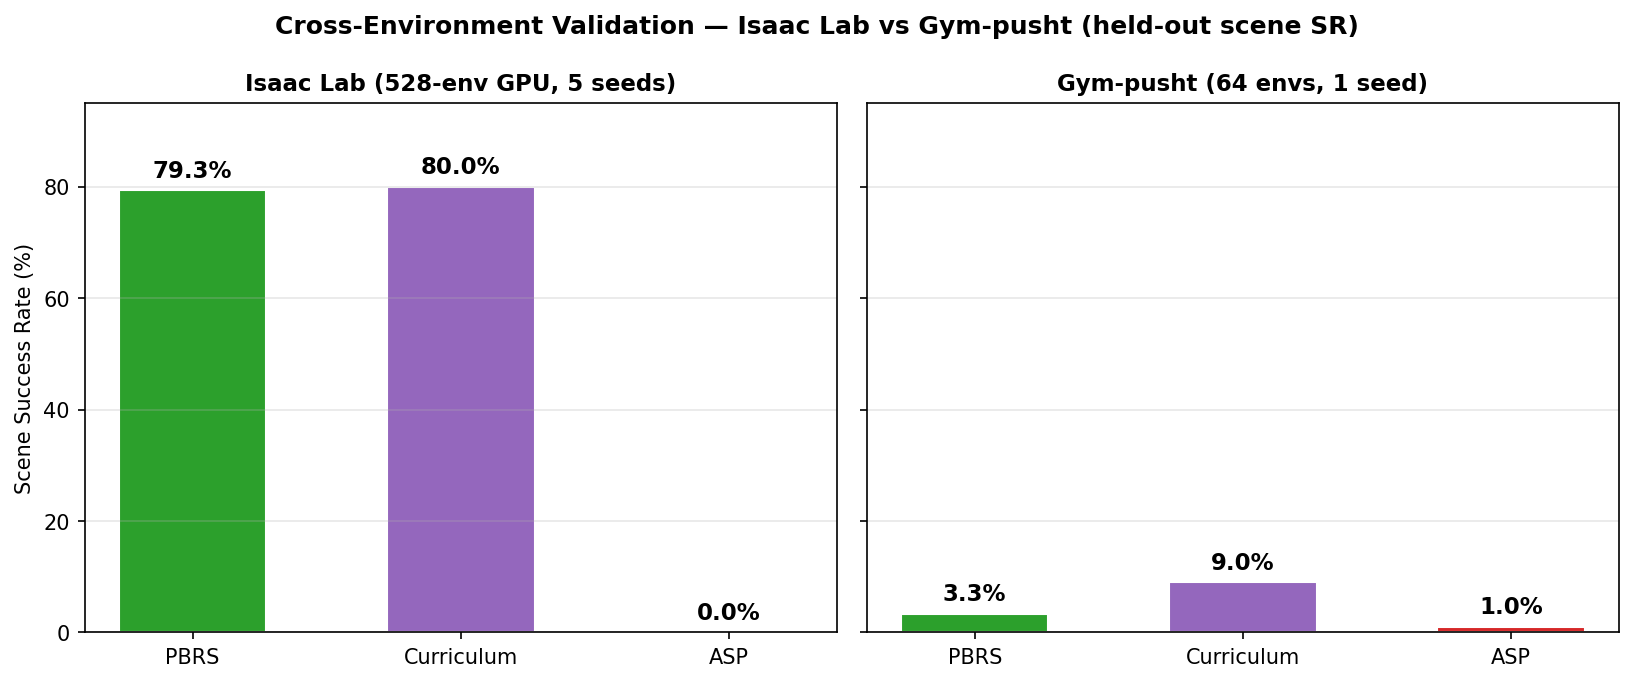
\includegraphics[width=0.96\textwidth]{figures/p1_sr_bars.png}

  \vspace{2pt}
  {\small The ordering single-agent $\approx$ curriculum $\gg$ self-play holds in both simulators.}

\end{frame}

% ~~~~~ SPEAKER NOTES ~~~~~
\note[itemize]{
\item Same models, same 30-scene thesis gate, two simulators. Left: Isaac (batch 7,920, 5 seeds). Right: gym-pusht (batch 960, 1 seed)
\item Isaac: PBRS 79.3\% $\approx$ Curriculum 80.0\% $\gg$ ASP 0.0\% — self-play transfers nothing
\item Gym: PBRS 3.3\%, Curriculum 9.0\%, ASP 1.0\% — the ordering holds, but absolute rates are far lower (fidelity + single seed)
\item Nuance: curriculum exceeds plain single-agent only at the small gym batch (9.0\% vs 3.3\%); at the Isaac batch they tie. The substitution is regime-dependent
}


\begin{frame}[t]{Per-Scene Outcomes — Isaac vs Gym}
  \centering
  
\includegraphics[width=1.0\textwidth]{figures/p3_heatmap.png}

  \vspace{2pt}
  {\small Colour: red (0.0) $\to$ yellow (0.5) $\to$ green (1.0). Numbers = fraction of trials passed per scene.}

\end{frame}

% ~~~~~ SPEAKER NOTES ~~~~~
\note[itemize]{
\item Per-scene fraction of trials passed across the 30 scenes: 5 Isaac models (PBRS, Curriculum, ASP-dPose, TASP-dPose, Bob-penalty) + gym-PBRS
\item Three blocks: rotation (1-10), position-only (11-20), pos+rot (21-30)
\item Isaac single-agent models (PBRS, Curriculum) fill most of the grid; the self-play models (ASP-dPose, TASP-dPose, Bob-penalty) are all 0.0 in every scene
\item gym-PBRS solves a single scene (3.3\%) — the pos+rot block is the universal bottleneck, and only the Isaac single-agent models clear it consistently
}


\sectionframe{7.\ Discussion}


\begin{frame}[t]{ASP Diagnostic — Alice \& Bob Training Dynamics}
  \centering
  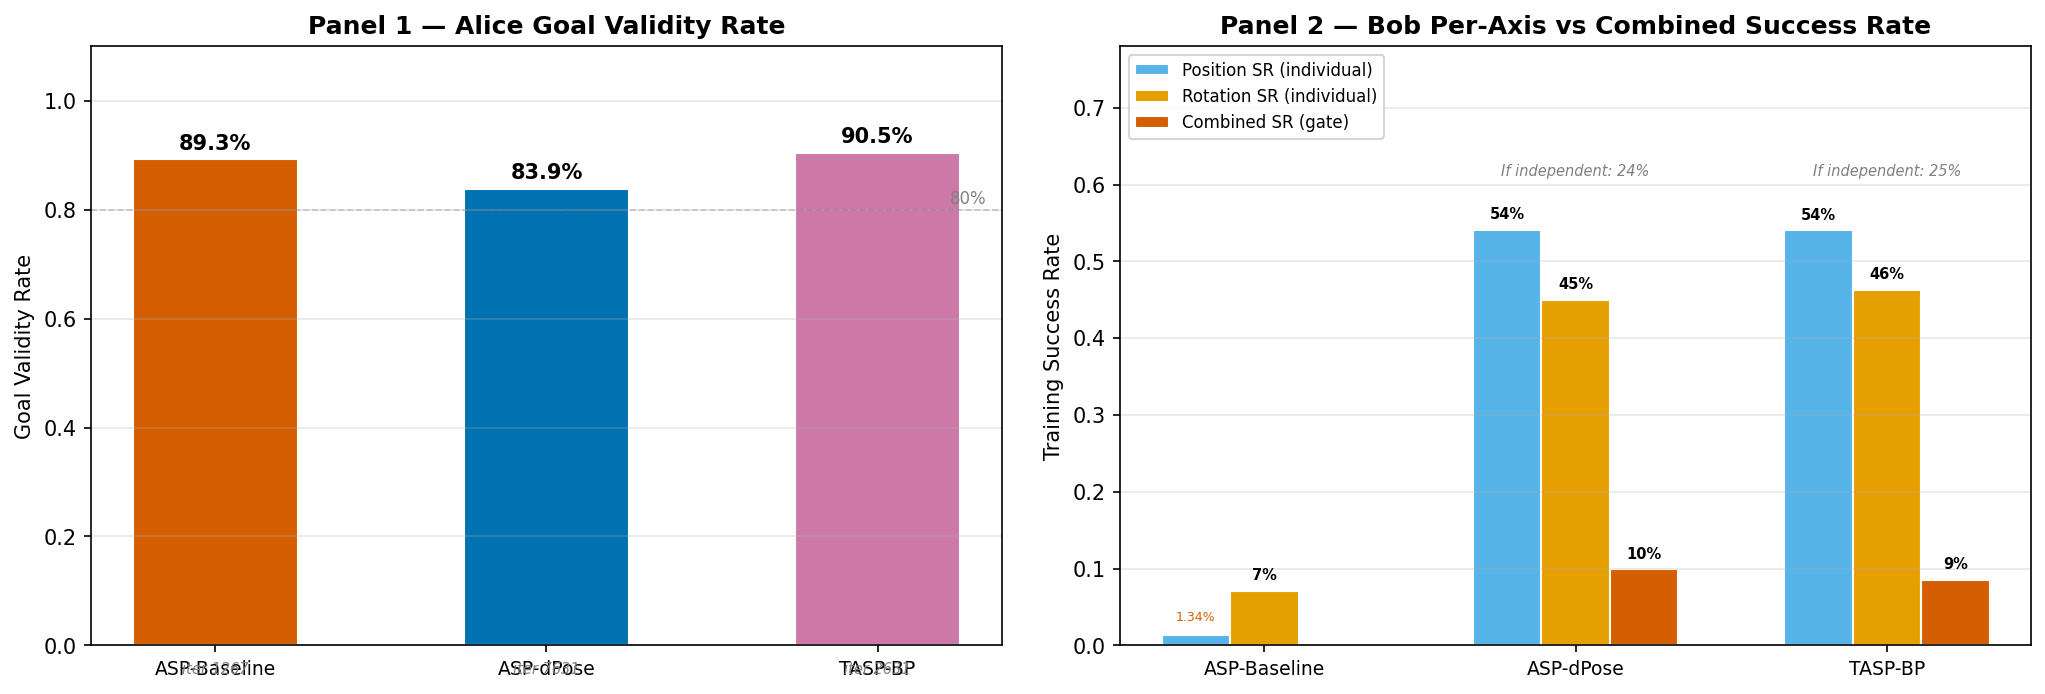
\includegraphics[width=\textwidth,height=0.72\textheight,keepaspectratio]{figures/asp_diagnostic_2panel.png}

  \vspace{2pt}
  {\small \textbf{Left:} Alice validity converges to 83--91\% across all three ASP variants at different training budgets. \textbf{Right:} Bob learns position and rotation to $\sim$50\% each under PBRS — but the combined gate caps at $\sim$10\%, 2.5$\times$ below the independence product.}
\end{frame}

% ~~~~~ SPEAKER NOTES ~~~~~
\note[itemize]{
\item Panel 1: Alice GoalValidityRate as a bar chart — ASP-Baseline 89\% (iter 1,267), ASP-dPose 84\% (iter 7,631), TASP-dPose-BP 91\% (iter 2,631). Alice learns across all variants despite different training budgets. Alice is NOT the problem.
\item Panel 2: Bob's training SR — per-axis vs combined gate. Under the original fractional reward, Bob learns nothing (PositionSR 1.3\%, Combined 0.07\%). With PBRS, Bob learns position to 54\% and rotation to 45--46\% individually — but the combined gate caps at 8.5--10.0\%. That's 2.5$\times$ below the independence product (24--25\%).
\item Key insight: PBRS provides enough gradient for Bob to learn each objective independently, but the adversarial goal distribution prevents simultaneous satisfaction of the coupled pos+rot gate. This is a causal bottleneck, not a measurement artifact (C4 resolved).
\item This explains the validation pattern: 20--40\% pos-only scene SR (Bob CAN do position alone), 0\% pos+rot scene SR (Bob CANNOT do both together under ASP).
}


\begin{frame}[t]{ASP — The Empirical Result}
  \textbf{No ASP configuration exceeds 16.7\% against an 80\% single-agent ceiling:}
  \vspace{2pt}
  \begin{center}
  \footnotesize
  \begin{tabular}{lcc}
    \toprule
    \textbf{ASP configuration} & \textbf{Valid SR} & \textbf{Pos+rot SR} \\
    \midrule
    Original fractional reward, 2{,}048 envs & 0.0\% & 0\% \\
    PBRS outcome-based (ASP-dPose) & 6.7\% & 0\% \\
    PBRS time-based (TASP-dPose) & \textcolor{hlred}{16.7\%} & 10\% \\
    PBRS time-based + Bob penalty & 0.0\% & 0\% \\
    gym-pusht (different sim, same gate) & 13.3\% & 0\% \\
    \midrule
    \rowcolor{hlgreen!15}
    \textbf{Single-agent ceiling (PPO-PBRS)} & \textbf{80.0\%} & \textbf{70\%} \\
    \bottomrule
  \end{tabular}
  \end{center}

  \vspace{2pt}
  {\small
  \begin{itemize}
    \item Self-play and single-agent cost the same per iteration ($\sim$0.022 it/s) — the gap is \textbf{structural}, not a budget artifact
  \end{itemize}
  }
\end{frame}

% ~~~~~ SPEAKER NOTES ~~~~~
\note[itemize]{
\item Across 5 ASP configurations, no variant exceeds 16.7\%; single-agent PPO-PBRS reaches 80.0\%
\item Time-based Alice (TASP-dPose) is the best ASP variant at 16.7\% — 2.5$\times$ better than outcome-based ASP-dPose (6.7\%), 10pp gain
\item Self-play and single-agent have identical per-iteration wall-clock (\textasciitilde0.022 it/s) — the 4.8$\times$ gap is structural, not a budget artifact
\item Pos+rot success remains near-zero for all ASP variants (0--10\%) — the combined gate is the unresolved bottleneck
\item The time-based Alice reward partially mitigates the adversarial dynamics by self-regulating toward solvable goals, but cannot close the gap
}

\sectionframe{8.\ Conclusion \& Takeaways}


\begin{frame}[t]{Conclusion — Self-Play vs Single-Agent (RQ1)}
  \begin{block}{\textbf{RQ1 — Self-play does not match single-agent training}}
    \small
    Single-agent: \textbf{79--80\,\%} held-out (5 seeds), every position-only scene solved. Self-play: \textbf{0.0\,\%} in every seed, every reward formulation, every environment count (256--2{,}048). A categorical failure to generalise.
  \end{block}

  \vfill\litfooter{[Plappert et al.\ 2021]~\textbf{[Sukhbaatar et al.\ 2018]}}
\end{frame}

% ~~~~~ SPEAKER NOTES ~~~~~
\note[itemize]{
\item RQ1: single-agent models solve 79--80\% of held-out scenes and every position-only scene; self-play models solve 0.0\% in every seed, under both Alice reward formulations, at every environment count from 256 to 2{,}048
\item The failure is categorical: not a small underperformance but a complete failure to transfer
}


\begin{frame}[t]{Conclusion — Which Setup Dimension (RQ2)}
  \begin{block}{\textbf{RQ2 — The coupled multi-objective gate is the factor}}
    \small
    The coupled gate turns the disc's \textbf{7.3\,\%} into \textbf{0.0\,\%} on the T-block. Compute scale, the imitation signal, and the goal representation contribute nothing: scale flat at zero; clip fraction 0.000.
  \end{block}

  \vfill\litfooter{[Plappert et al.\ 2021]~\textbf{[Sukhbaatar et al.\ 2018]}~[Berner et al.\ 2019]}
\end{frame}

% ~~~~~ SPEAKER NOTES ~~~~~
\note[itemize]{
\item RQ2: five dimensions isolated one at a time: goal coupling, reward formulation, imitation signal, goal representation, compute scale
\item Ruled out by experiment: compute scale (8$\times$ batch flat at zero), imitation signal (clip fraction 0.000, never flows), goal representation (ablation unchanged)
\item The coupled gate is the factor: it reduces the disc's residual 7.3\% to the T-block's 0.0\%
}


\begin{frame}[t]{Ablations — Per-Scene Outcomes (RQ2)}
  \centering
  \includegraphics[width=1.0\textwidth]{figures/ablation_heatmap.png}

  \vspace{2pt}
  {\small Colour: red (0.0) $\to$ yellow (0.5) $\to$ green (1.0). Removing ABC or the goal encoder does not change self-play's 0.0\,\%; the disc positive control is unchanged (6.7\,\%).}

\end{frame}

% ~~~~~ SPEAKER NOTES ~~~~~
\note[itemize]{
\item Per-scene fraction of trials passed for the ablation arms: rows 1--5 on the 30 T-block scenes, rows 6--8 on the 30 disc scenes
\item Removing ABC or the goal encoder leaves the T-block self-play models at 0.0\%: the ablations change nothing
\item The disc positive control is unchanged at 6.7\%: imitation helps only where the task is already easy, and not at all in the discrete macro-action space
}


\begin{frame}[t]{Conclusion — Mechanism (RQ3)}
  \begin{block}{\textbf{RQ3 — A generalisation failure, not a skill-composition failure}}
    \small
    Self-play logs \textbf{77.9\,\%} (disc) and \textbf{35.8\,\%} (T-block) training-time success; none transfers. The value function is stale under the non-stationary goal distribution: a generalisation failure, not a skill-composition failure.
  \end{block}

  \vfill\litfooter{[Plappert et al.\ 2021]~\textbf{[Sukhbaatar et al.\ 2018]}~[Schulman et al.\ 2017]}
\end{frame}

% ~~~~~ SPEAKER NOTES ~~~~~
\note[itemize]{
\item RQ3: self-play logs substantial training-time success (77.9\% disc, 35.8\% T-block) but transfers none; the competence is confined to the goals Alice's own curriculum produces
\item Single-agent moves in the opposite direction: a per-push training rate of $\sim$11\% rises to 79\% under the held-out evaluation budget
\item The mechanism is a generalisation gap driven by the value-function bias under the shifting goal distribution: not a failure to compose two individually learned skills
}


\begin{frame}[t]{Conclusion — Reward Efficiency (Supporting RQ)}
  \begin{block}{\textbf{Supporting RQ — PBRS solves the task; efficiency comparison pending}}
    \small
    PBRS solves \textbf{79.3\,\%} of held-out scenes (5 seeds); policy invariance (Ng et al.\ 1999) holds under stochastic PhysX. The efficiency comparison against the improvement reward is pending.
  \end{block}

  \vfill\litfooter{[Ng et al.\ 1999]~[Grze\'s 2017]~[Harutyunyan et al.\ 2015]}
\end{frame}

% ~~~~~ SPEAKER NOTES ~~~~~
\note[itemize]{
\item Supporting RQ: PBRS reaches 79.3\% held-out SR at 528 envs, confirming the Ng (1999) policy-invariance guarantee survives contact-rich stochastic PhysX
\item The reward-efficiency comparison against the improvement reward (PPO-Baseline) is still training at writing time: its held-out validation is pending
}


\begin{frame}[t]{Computational Overhead — Self-Play Is Not Slower}
  \textbf{Controlled measurement} (same machine, same 528 envs, same cuRobo IK + physics): \\
  PPO-PBRS (single-agent) vs the self-play variants run at \textcolor{hlgreen}{\textbf{$\sim$1.0$\times$}} per-iteration wall-clock ($\sim$0.022 it/s for both). The 2-agent machinery (Alice + Bob, GoalEncoder, ABC, historical pool) adds \textbf{no} measurable per-iteration overhead — the shared cuRobo IK + PhysX contact step dominates the cost.

  \vspace{4pt}
  \textbf{Key result:}
  \begin{itemize}
    \item Self-play is \textbf{not} slower per iteration — it simply \textbf{does not learn}
    \item The real cost of self-play is model/code complexity and added failure modes (two networks, non-stationary objective, ABC), \emph{not} throughput
    \item So the 4.8$\times$ performance gap is \textbf{not} a compute-budget artifact — both used the same compute
  \end{itemize}

  \vfill\litfooter{[Plappert et al.\ 2021]~[Schulman et al.\ 2017]}
\end{frame}

% ~~~~~ SPEAKER NOTES ~~~~~
\note[itemize]{
\item Controlled, same-machine measurement: self-play and single-agent run at identical iteration cost (~0.022 it/s) on the same 528-env GPU setup. The 2-agent machinery adds ~no per-iteration wall-clock because cuRobo IK and physics dominate
\item I deliberately do NOT claim a 5–10× self-play overhead — there is no controlled measurement supporting that; the only honest number is ~1.0× per iteration
\item Key distinction: self-play doesn't fail because it's computationally expensive per iteration. It fails because it doesn't learn. The two are separate problems
\item The measured Isaac-vs-gym throughput (~172 push/s vs ~22 push/s for self-play on CPU) is shown in the Isaac Lab venue slide (Evaluation) — establishing that Isaac Lab is the right venue, not a handicap
}


\begin{frame}[t]{Limitations \& Future Work}
  \small
  \begin{enumerate}
    \item \textbf{Bob penalty collapses to 0\%} — penalty on catastrophe phase ends creates a ``fail-fast'' equilibrium.\\
    $\rightarrow$ \textbf{Zero-sum game theory} (Letcher 2019) may stabilise symmetric self-play; test penalty only on non-catastrophe ends.

    \item \textbf{Combined pos+rot gate is the universal bottleneck} — joint gate rarely fires under self-play (0--10\% pos+rot).\\
    $\rightarrow$ \textbf{Relaxed success gate} or partial credit per objective to provide gradient toward both.

    \item \textbf{Single-seed validation} — training SR variance across 5 chains (BestSR 0.081--0.110).\\
    $\rightarrow$ \textbf{Re-evaluate} checkpoints across 5 seeds for validation confidence intervals.

    \item \textbf{Curriculum substitution is regime-dependent} — PBRS substitutes for curriculum at batch 7{,}920; curriculum helps at batch 960.\\
    $\rightarrow$ \textbf{Batch-size sweep} to map the substitution boundary and gradient-variance threshold.
  \end{enumerate}

  \vfill\litfooter{[Letcher et al.\ 2019]~[Dennis et al.\ 2020]~[Schulman et al.\ 2017]}
\end{frame}

% ~~~~~ SPEAKER NOTES ~~~~~
\note[itemize]{
\item Four paired limitation→future-work items: (1) Bob penalty collapse → zero-sum game theory as stabiliser, (2) combined gate bottleneck → relaxed success criteria, (3) single-seed validation → multi-seed re-evaluation, (4) regime-dependent RQ3 → systematic batch-size sweep
\item These are concrete because each limitation is an empirical finding; each future-work direction is a specific experiment, not a vague aspiration
\item The take-home: PBRS single-agent at 80\% is the practical recommendation; the remaining open questions are about when and why to add complexity — the testable gaps, not the unknown unknowns
}

\makefinalpage

% ============================================================
% APPENDIX SLIDES
% ============================================================

% ============================================================
% APPENDIX
% ============================================================
\appendix
\begin{frame}[t]{Appendix Outline}
  \begin{itemize}
    \item A. Push Mechanics — Limit Surface \& Characteristic Length $L$
    \item B. Training curves for all PBRS models (Success Rate, Reward, Loss)
    \item C. PBRS parameter sensitivity ($k_p$, $k_r$, $w_{\text{pos}}$, $w_{\text{rot}}$)
    \item D. Validation scene descriptions (30 test cases)
    \item E. cuRobo IK pipeline and workspace configuration
    \item F. Observation space specifications (all model variants)
    \item G. Per-test error bars — PPO-PBRS vs PPO-Curriculum head-to-head and all-model comparison (95\% binomial CIs)
    \item \textbf{H. P82 Curriculum Trigger Bug} — why the original trigger never fired
    \item \textbf{I. BobPenalty Fail-Fast Equilibrium} — degeneracy mechanism
    \item \textbf{J. Confounded Ablation Disaggregation} — 7-axis variation table
    \item \textbf{K. Training Budget Comparison} — envs, iterations, push-macros
    \item \textbf{L. Validation Protocol} — scene set, trials, disclosed limitations
  \end{itemize}
\end{frame}


\begin{frame}[t]{PBRS — The Shaping Theorem}
  \textbf{Ng et al.:}
  \[
  \boxed{\mathcal{R}'(s,a,s') = \mathcal{R}(s,a,s') + \underbrace{\gamma\Phi(s') - \Phi(s)}_{\text{shaping reward }F}}
  \]
  \textbf{Policy invariance:} $Q'(s,a) = Q(s,a) - \Phi(s)$ — optimal actions unchanged.

  \vspace{4pt}
  \textbf{Our potential functions (PPO-PBRS / PPO-Curriculum):}
  \[
  \Phi(s) = w_{\text{pos}} e^{-k_p d_{\text{pos}}^2} + w_{\text{rot}} e^{-k_r c(s)},\quad
  c(s) = \frac{1-\cos(\theta^*-\theta)}{2}
  \]
  $k_p{=}30,\; k_r{=}5,\; w_{\text{pos}}{=}w_{\text{rot}}{=}10.0$\\
  \textbf{Dense reward:} $F(s,s') = \Phi(s') - \Phi(s)$  —  difference only, no constant drain.

  \vspace{4pt}
  \textbf{Episodic PBRS} : $\gamma_{\text{shaping}}{=}1.0$ valid — $\sum F = \Phi(s_T)-\Phi(s_0)$ bounded.

  \vfill\litfooter{[Ng, Harada \& Russell 1999]~\textbf{[Grze\'s 2017]}~[Devlin \& Kudenko 2012]}
\end{frame}

% ~~~~~ SPEAKER NOTES ~~~~~
\note[itemize]{
\item The fundamental theorem: add F = gamma·Phi(s') − Phi(s) without changing optimal policies
\item Proof sketch: Q'(s,a) = Q(s,a) − Phi(s). Since Phi(s) depends on state only (not action), argmax unchanged
\item Our potential: sum of two exponentiated distance functions. Cosine c(s) respects S¹ topology — no discontinuity at ±π
\item Episodic PBRS: gamma_shaping=1.0 is valid — sum over an episode is bounded = Phi(s_T) − Phi(s_0)
}


\begin{frame}[t]{PBRS — Why It's the Right Choice}
  \textbf{Properties of $F(s,s') = \Phi(s') - \Phi(s)$:}
  \begin{enumerate}
    \item \textbf{Markovian} — depends only on $s,s'$, not history. 
    \item \textbf{Bounded} — exponential potentials prevent reward explosions from PhysX contact spikes.
    \item \textbf{Zero-sum cycles} — detour pushes net to zero; agent free to explore without reward hacking.
    \item \textbf{No constant drain} — $F{=}0$ when stationary; no penalty for hesitation or deliberation.
  \end{enumerate}

  \vspace{4pt}
  \textbf{Key consequence:} you can replace any ad-hoc reward with a potential-based one \emph{without changing what the agent learns} — only \emph{how fast} it learns. Reward design and policy optimisation are decoupled.

  \vfill\litfooter{[Ng, Harada \& Russell 1999]~\textbf{[Grze\'s 2017]}~[Harutyunyan et al.\ 2015]}
\end{frame}

% ~~~~~ SPEAKER NOTES ~~~~~
\note[itemize]{
  \item Old formula violated this by dividing by $d_{\text{prev}}$.
\item Four properties that make PBRS ideal for contact-rich pushing: Markovian (depends only on s,s'), Bounded (exponentials cap reward range), Zero-sum cycles (detour pushes give zero net F — no reward hacking), No constant drain (stationary agent gets F=0)
\item The old fractional improvement formula violated all four — non-Markov (divides by d_prev), unbounded (division by 0.01), negative-sum (staying still was penalised)
}


\begin{frame}[t]{PPO-PBRS — Training Dynamics}
  \begin{center}
    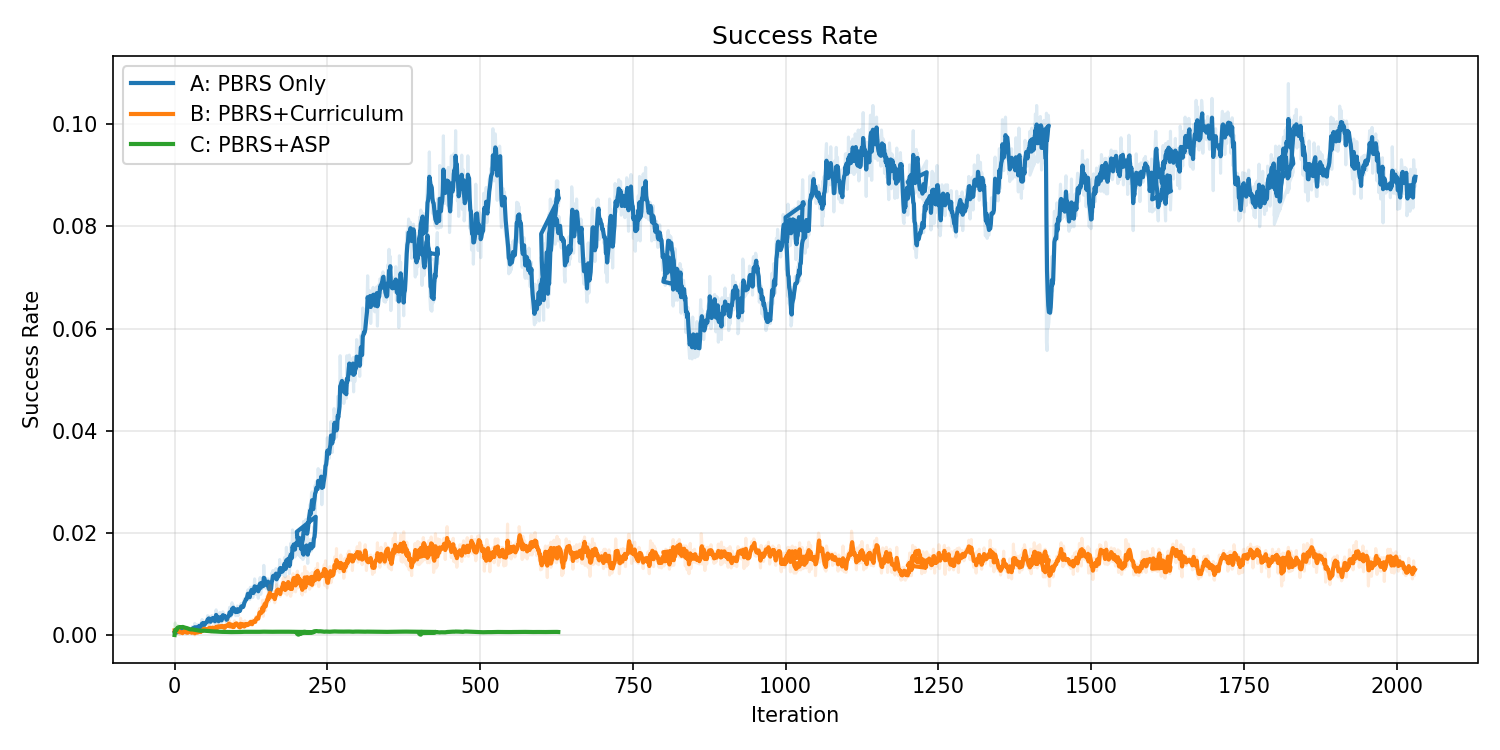
\includegraphics[width=0.48\textwidth]{figures/cmp_Success_Rate.png}
    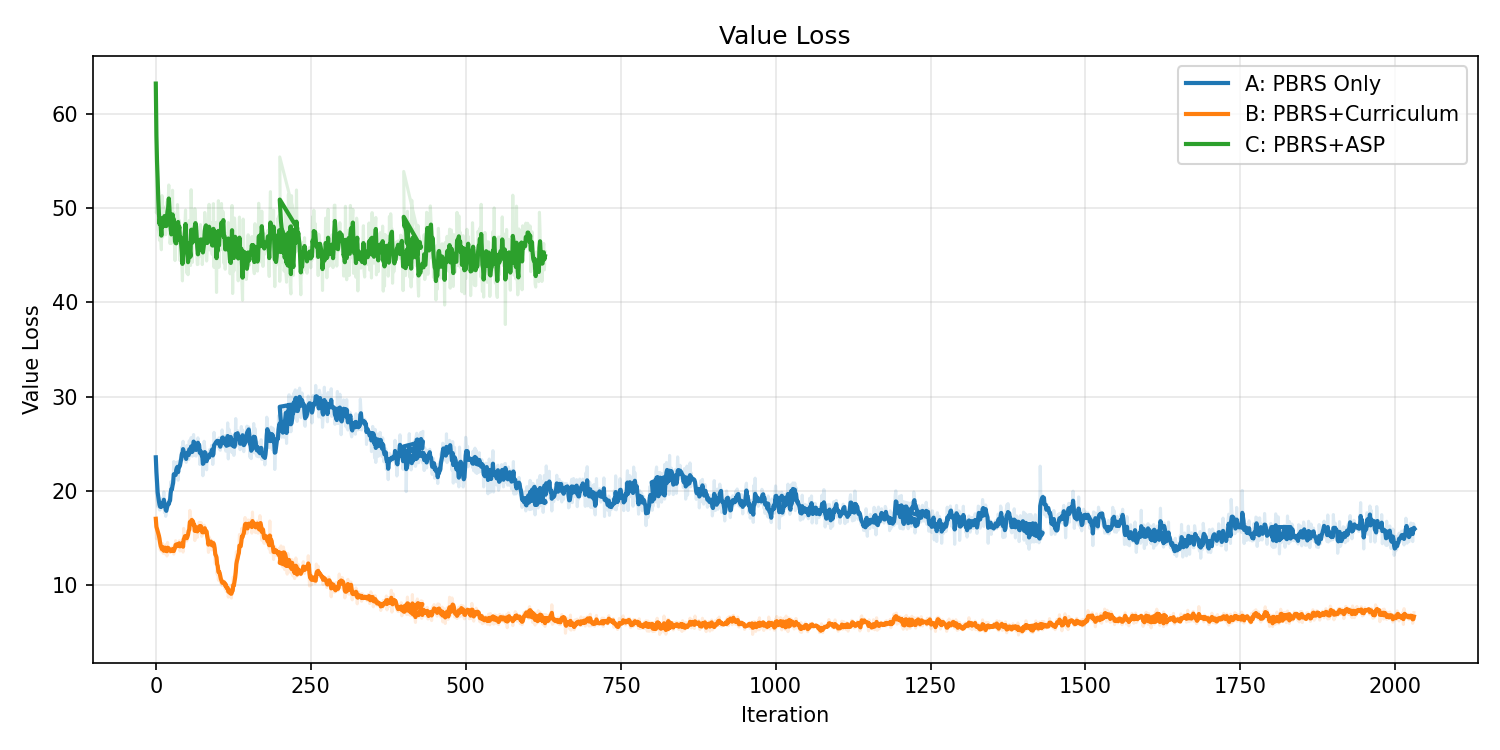
\includegraphics[width=0.48\textwidth]{figures/cmp_Value_Loss.png}
  \end{center}

  \vspace{2pt}
  {\small \textbf{Left:} PPO-PBRS (blue) steadily improves training success rate over 3000 iterations. PPO-Curriculum (orange) follows a similar trajectory but converges slightly lower. Self-play variants remain near baseline throughout. \textbf{Right:} Stable value function — no explosion. Initial $V\approx0.057$ with gain$=0.01$.}

  \vfill\litfooter{[Schulman et al.\ 2017]~[Ng et al.\ 1999]}
\end{frame}

% ~~~~~ SPEAKER NOTES ~~~~~
\note[itemize]{
\item Left plot: training success rate over ~3000 iterations. PPO-PBRS (blue) improves from near-zero to ~9.4\% (strict combined gate). PPO-Curriculum (orange, P82-fixed) follows a similar trajectory. Self-play variants remain near baseline
\item Right plot: value loss stays stable — no explosion. The PBRS exponential potentials prevent the reward spikes that caused GAE chain reactions and critic instability in earlier attempts
}


\begin{frame}[t]{PPO-Curriculum vs PPO-PBRS}
  \begin{center}
  \footnotesize
  \begin{tabular}{lccc}
    \toprule
    \textbf{Metric} & \textbf{PPO-PBRS} & \textbf{PPO-Curriculum} & \textbf{Gap} \\
    \midrule
    Validation SR & \textcolor{hlgreen}{\textbf{80.0\%}} & 76.7\% & 1.04$\times$ \\
    PosErr (m) & 0.032 & \textcolor{hlgreen}{\textbf{0.023}} & B 28\% lower \\
    RotErr (rad) & 0.568 & 0.663 & A 14\% lower \\
    Pos-only SR & 100\% & 100\% & equal \\
    Pos+rot SR & 70\% & 65\% & 5pp \\
    \bottomrule
  \end{tabular}
  \end{center}
  \vspace{1pt}
  {\scriptsize \textbf{Result:} Curriculum improves position precision (0.023 vs 0.032 m) from the pos-only phase, but slightly degrades rotation (0.663 vs 0.568 rad). Net effect: B is 3.3pp behind A.}
  {\scriptsize \textbf{Statistical note:} The 3.3pp A vs B gap is \textbf{not} significant (p\,$>$\,0.05, two-tailed z-test; SE of difference = ±10.6pp across 30 independent scenes). Both A and B solve the task similarly well.}
  {\scriptsize \textbf{Takeaway:} A staged curriculum \emph{can} work alongside PBRS, but does not beat the simpler no-curriculum baseline.}

  \vfill\litfooter{[Narvekar et al.\ 2020]~[Portelas et al.\ 2020]~[Florensa et al.\ 2017]}
\end{frame}

% ~~~~~ SPEAKER NOTES ~~~~~
\note[itemize]{
\item Head-to-head on identical 30 T-block scenes: PPO-PBRS 80.0\% vs PPO-Curriculum 76.7\%
\item PPO-Curriculum actually beats PPO-PBRS on position precision (0.023 vs 0.032 m) — the pos-only Phase 1 training produces tighter position control. But rotation is slightly worse (0.663 vs 0.568 rad)
\item Both achieve 100\% pos-only SR. The combined pos+rot gate is 70\% (PPO-PBRS) vs 65\% (PPO-Curriculum)
\item The curriculum is functional but fails to outperform the simpler baseline. Adding structure adds complexity without adding net value
}


\begin{frame}[t]{Self-Play — Validation Comparison}
  \begin{center}
  \begin{tabular}{lccc}
    \toprule
    \textbf{Model} & \textbf{Valid SR} & \textbf{PosErr} & \textbf{RotErr} \\
    \midrule
    \rowcolor{hlgreen!15}
    \textbf{PPO-PBRS} (single-agent, ref.) & \textbf{80.0\%} & 0.032 m & 0.568 rad \\
    \midrule
    \textbf{TASP-dPose} (time-based) & \textbf{16.7\%} & 0.158 m & 1.457 rad \\
    \textbf{ASP-dPose} (outcome-based) & 6.7\% & 0.143 m & 1.612 rad \\
    \bottomrule
  \end{tabular}
  \end{center}

  \vspace{4pt}
  {\small \textbf{Key findings:}}
  \begin{itemize}
    \item Time-based self-play (TASP-dPose) is 2.5$\times$ better than outcome-based (ASP-dPose), but still \textbf{4.8$\times$ below} single-agent PPO-PBRS
    \item No self-play variant achieves pos+rot SR above 10\% — the combined gate remains the bottleneck
    \item Self-play complexity provides no benefit

  \end{itemize}

  \vfill\litfooter{[Plappert et al.\ 2021]~\textbf{[Sukhbaatar et al.\ 2018]}~[Dennis et al.\ 2020]}
\end{frame}

% ~~~~~ SPEAKER NOTES ~~~~~
\note[itemize]{
\item PPO-PBRS (single-agent, reference) at 80.0\% vs TASP-dPose (best self-play variant) at 16.7\% — 4.8× gap
\item Time-based Alice (TASP-dPose) partially corrects the adversarial curriculum by rewarding solvable goals — gains 10pp over ASP-dPose
\item But even the best self-play variant cannot close the gap. The self-play dynamics prevent learning the combined pos+rot objective
\item Both self-play variants trained identically (528 envs, ∼3000 iters, PBRS dense reward for Bob) — the only difference is Alice's reward structure
}


\begin{frame}[t]{Comparison Summary — Per-Scene Position $\times$ Rotation Error}
  \begin{center}
    
\includegraphics[width=0.8\textwidth]{figures/plot3_failure_taxonomy.png}
  \end{center}

  \vspace{4pt}
  {\small \textbf{Three observations from the success rectangle (pos$<$5\,cm, rot$<$0.2\,rad):}
  \begin{itemize}
    \item \textbf{PPO-PBRS} (left): 24/30 scenes land inside the green box — solves position and rotation on nearly all scenes.
    \item \textbf{PPO-Curriculum} (center): position errors tightly cluster under 5\,cm (Phase-1 training); rotation is the bottleneck, with RotErr $>$ 0.2 for most pos+rot scenes.
    \item \textbf{ASP-dPose} (right): only 2 successes — points scatter far outside, with RotErr $>$ 1.4\,rad. Rotation is never learned.
  \end{itemize}}

  \vfill\litfooter{[Ng et al.\ 1999]~[Grze\'s 2017]~[Plappert et al.\ 2021]}
\end{frame}

% ~~~~~ SPEAKER NOTES ~~~~~
\note[itemize]{
\item Three-panel scatter: each point is one held-out scene — position error vs rotation error; the green box is the success region (pos < 5\,cm, rot < 0.2\,rad). PPO-PBRS fills it; PPO-Curriculum clusters position inside it but rotation outside it; ASP-dPose scatters far out.
\item The curriculum forces consistent position control from Phase-1 but cannot fix the combined pos+rot gate; self-play fails both axes.
}


\begin{frame}[t]{Appendix A — Push Mechanics: Limit Surface \& $L$}
  \begin{columns}[T,onlytextwidth]
    \begin{column}{0.46\textwidth}\small
      \textbf{Limit surface normality}: $\mathbf{t} \propto \nabla f(\mathbf{w})$ — twist is normal to the surface, so every push couples translation \emph{and} rotation.

      \vspace{2pt}
      \textbf{Characteristic length $L$} (radius of gyration):
      \begin{itemize}
        \item \textbf{T-block} $L=0.07$\,m — an off-centre push couples translation \emph{and} rotation
        \item $L$ is a physical constant, \emph{not} a hyperparameter
      \end{itemize}
    \end{column}
    \begin{column}{0.52\textwidth}
      \centering
      
\includegraphics[width=0.85\textwidth]{figures/diagram_limit_surface.png}\\[2pt]
      {\scriptsize The T-block rotates under an off-centre push (coupled SE(2) motion)}
    \end{column}
  \end{columns}

  \vfill\litfooter{[Goyal et al.\ 1991]~[Howe \& Cutkosky 1996]~[Mason 1986]}
\end{frame}


\begin{frame}[t]{Appendix B — Training Curves (All PBRS Models)}
  \begin{columns}[T]
    \begin{column}{0.48\textwidth}
      \centering
      \textbf{Success Rate}
      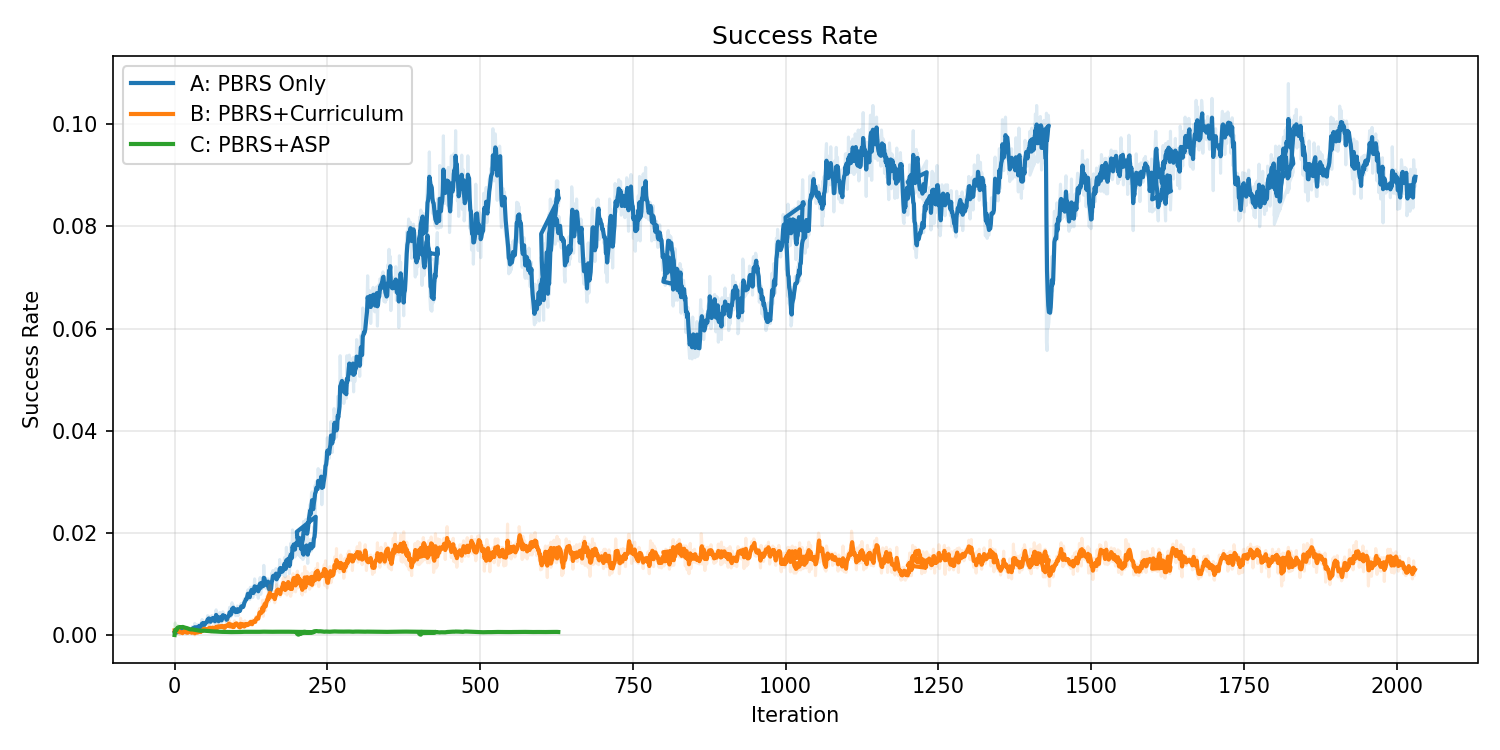
\includegraphics[width=0.72\textwidth]{figures/cmp_Success_Rate.png}
    \end{column}
    \begin{column}{0.48\textwidth}
      \centering
      \textbf{Mean Reward}
      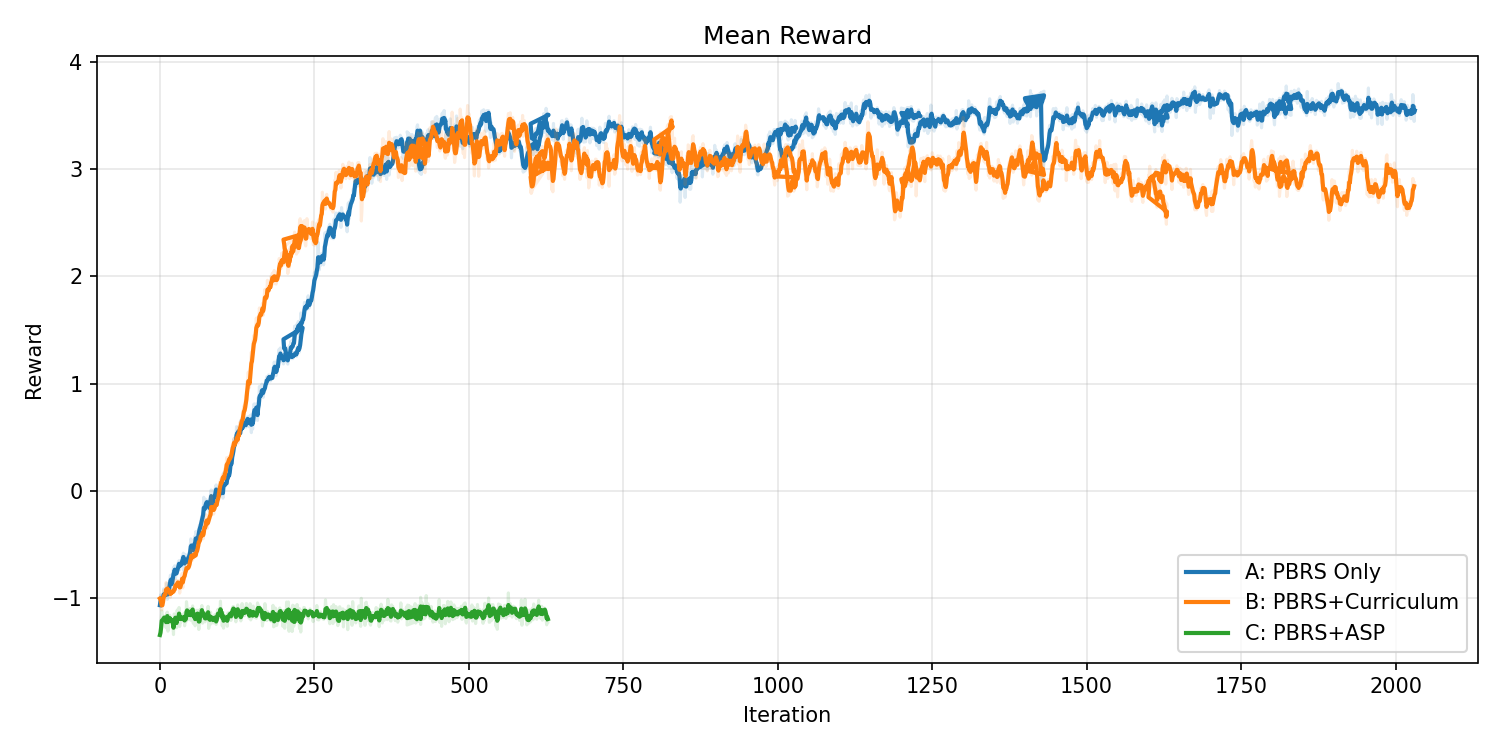
\includegraphics[width=0.72\textwidth]{figures/cmp_Mean_Reward.png}
    \end{column}
  \end{columns}

  \vspace{2pt}
  \begin{columns}[T]
    \begin{column}{0.48\textwidth}
      \centering
      \textbf{Policy Loss}
      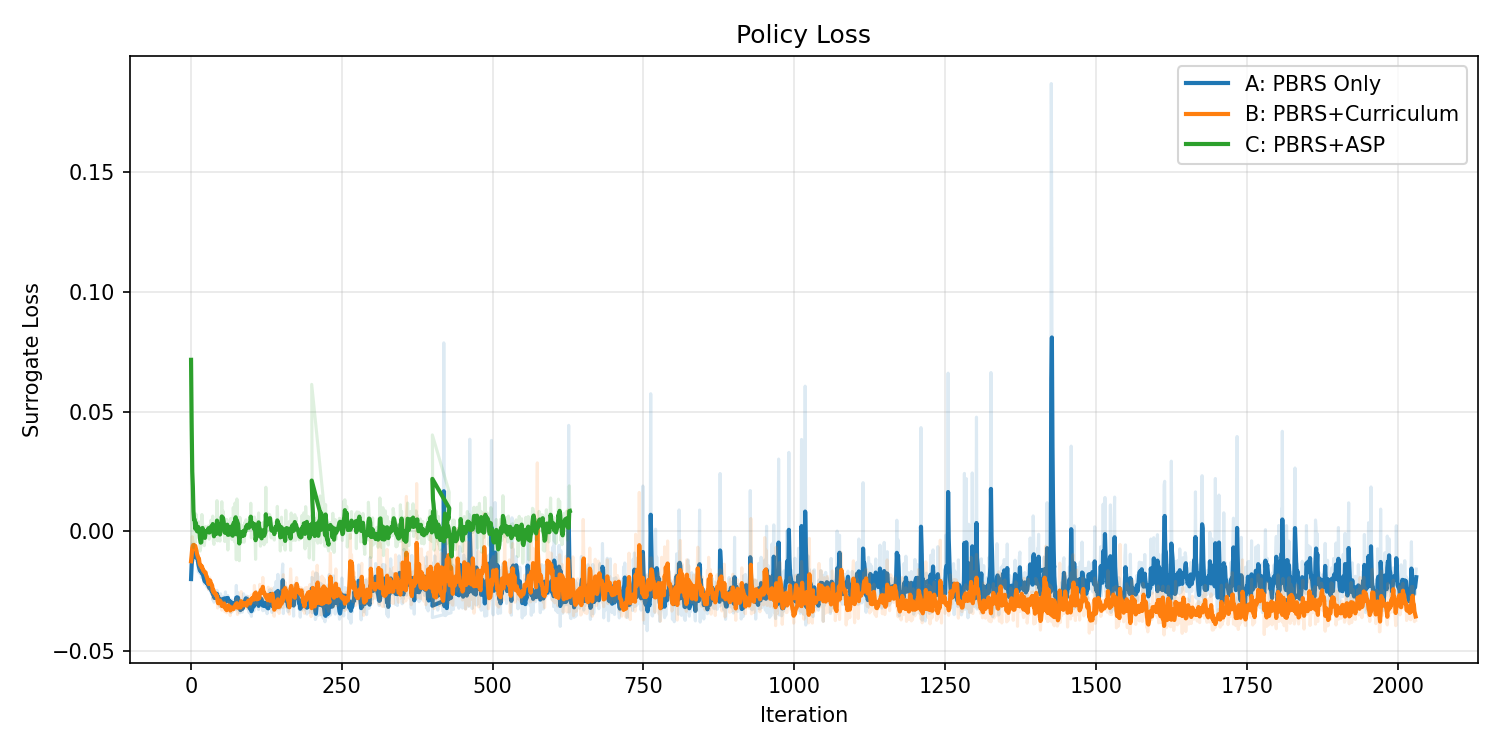
\includegraphics[width=0.72\textwidth]{figures/cmp_Policy_Loss.png}
    \end{column}
    \begin{column}{0.48\textwidth}
      \centering
      \textbf{Value Loss}
      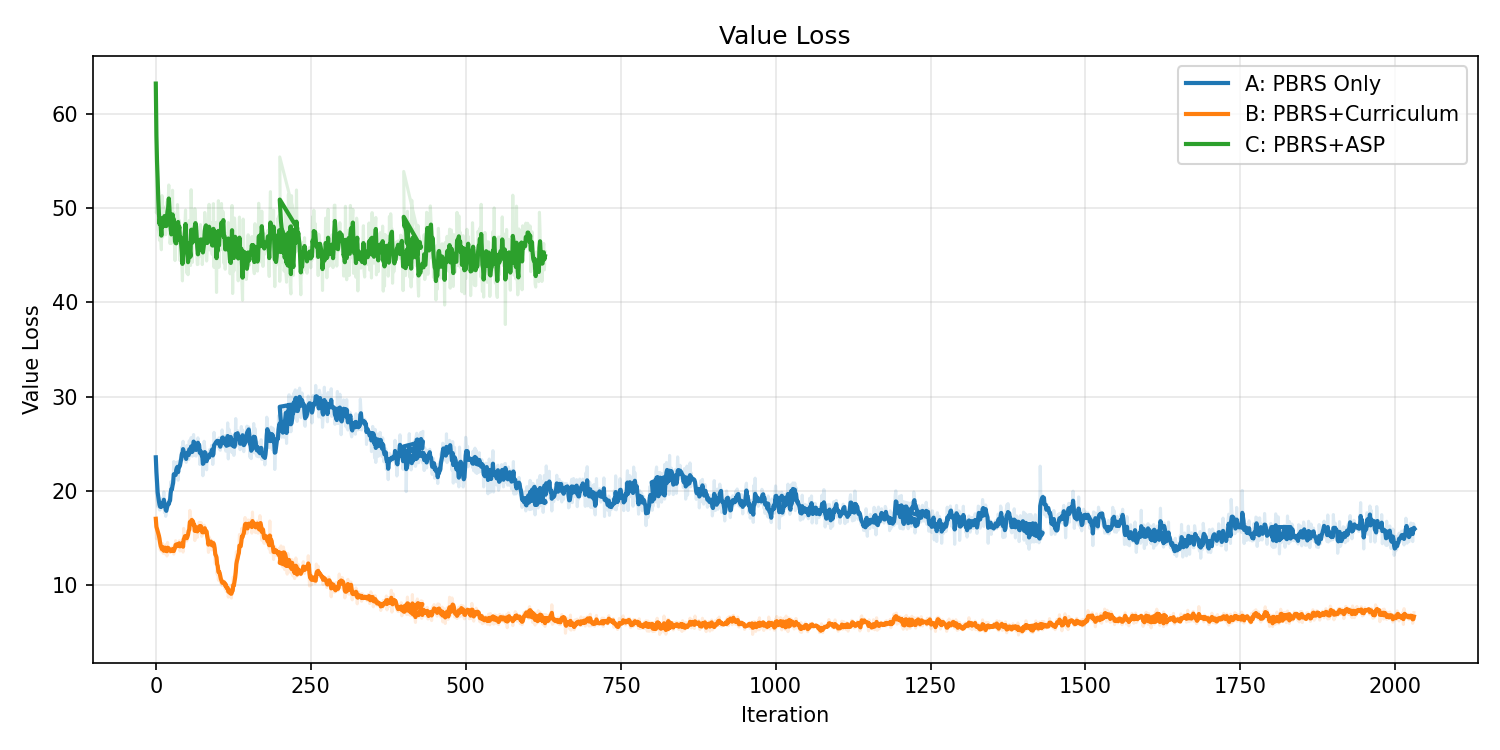
\includegraphics[width=0.72\textwidth]{figures/cmp_Value_Loss.png}
    \end{column}
  \end{columns}
\end{frame}


\begin{frame}[t]{Appendix C — PBRS Theory Analysis}
  \begin{columns}[T]
    \begin{column}{0.48\textwidth}
      \centering
      \textbf{Potential Landscape} \\
      $\Phi(s) = w\cdot\exp(-k\cdot d^2)$
      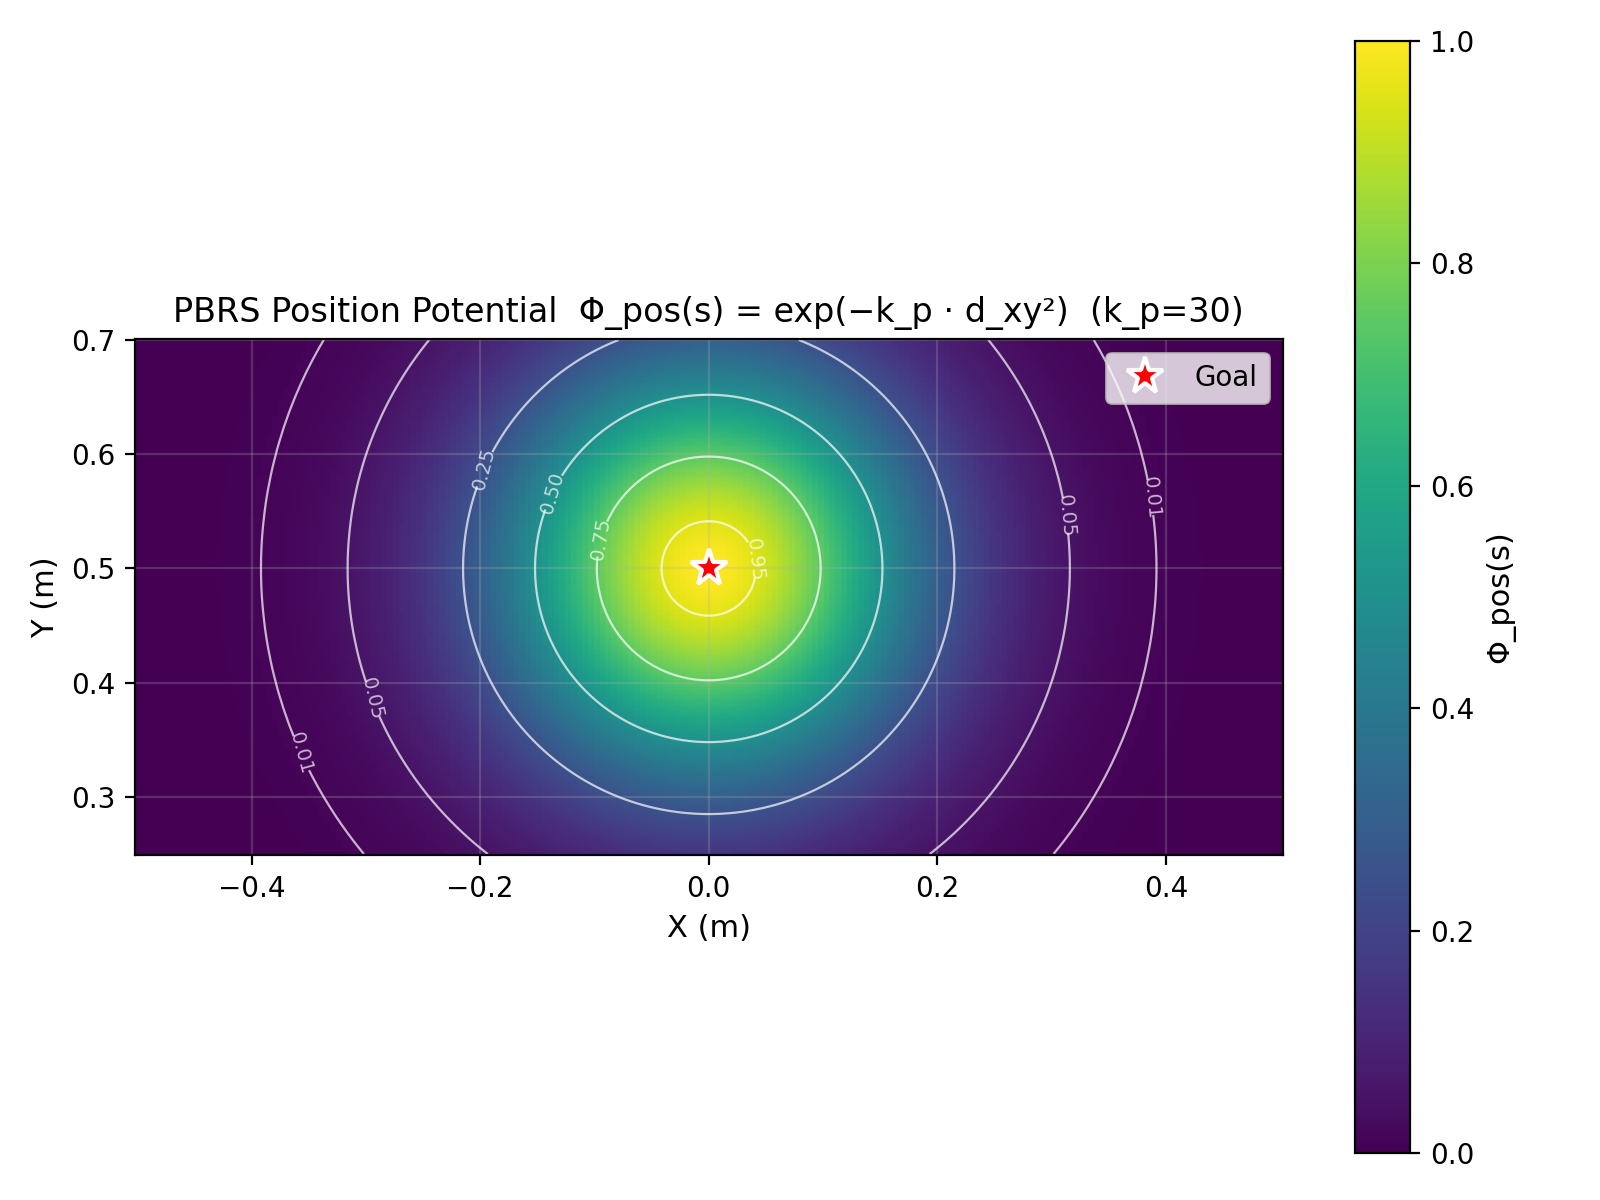
\includegraphics[width=0.52\textwidth]{figures/a1_potential_landscape.png}
    \end{column}
    \begin{column}{0.48\textwidth}
      \centering
      \textbf{Gradient Comparison} \\
      PBRS vs Fractional Formula
      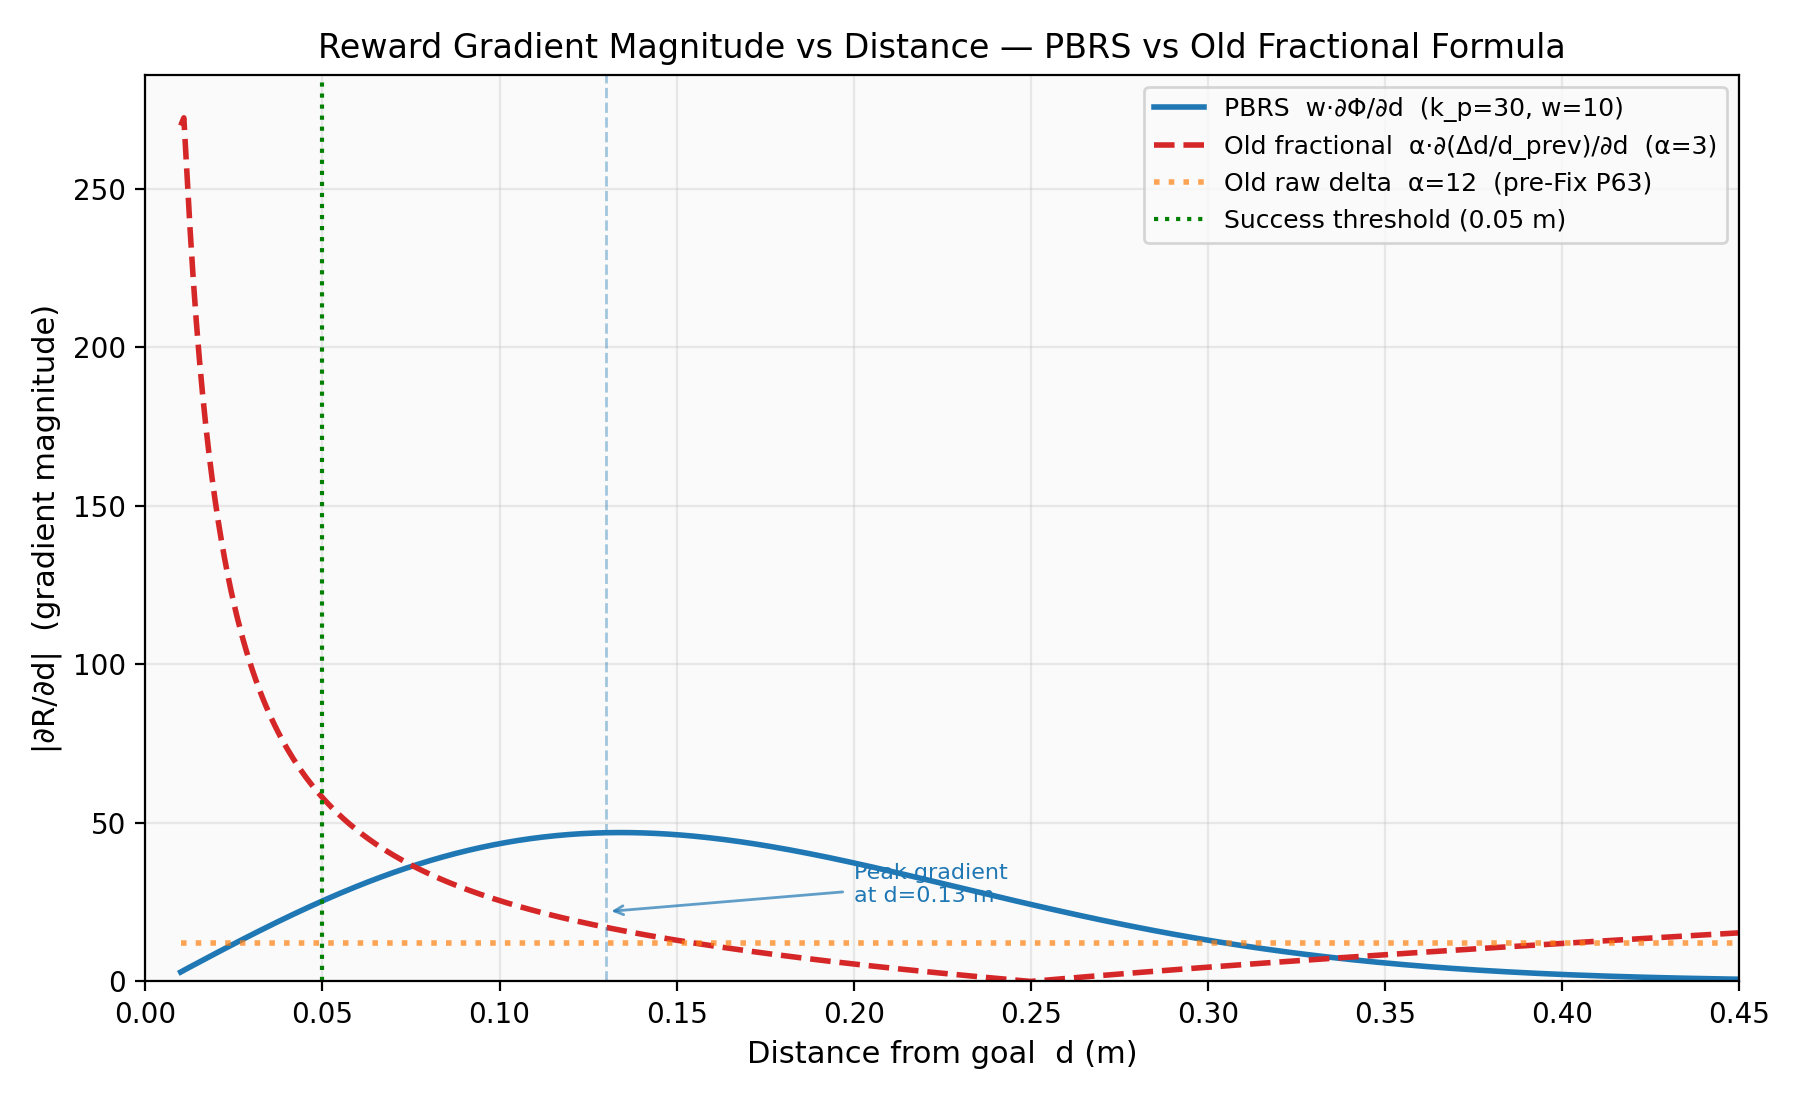
\includegraphics[width=0.52\textwidth]{figures/a2_gradient_comparison.png}
    \end{column}
  \end{columns}

  \vspace{2pt}
  \begin{center}
    \textbf{Cosine Angular Distance} $c(s) = (1-\cos(\theta^*-\theta))/2$
    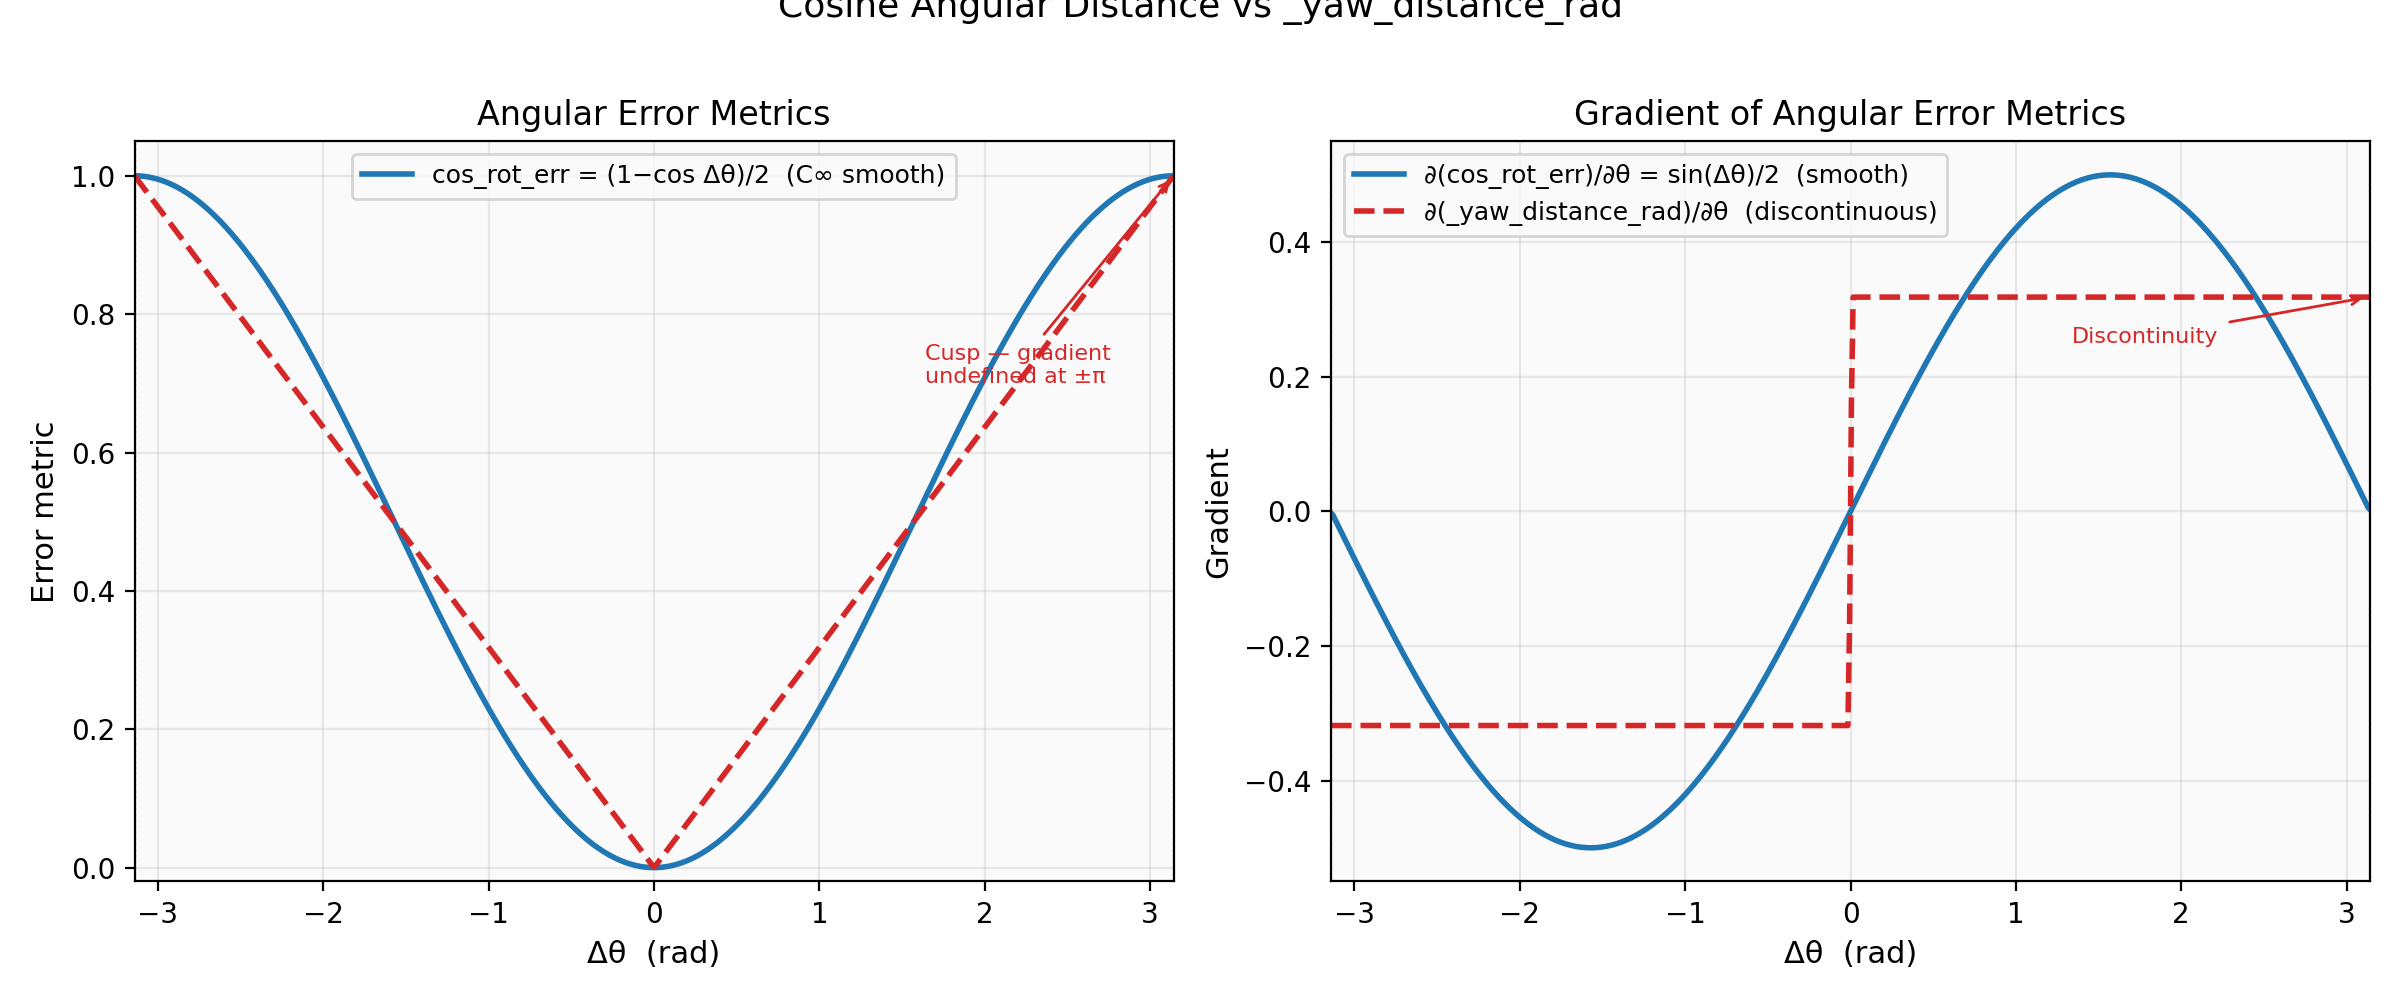
\includegraphics[width=0.30\textwidth]{figures/a4_cosine_distance.png}
  \end{center}
\end{frame}


\begin{frame}[t]{Appendix G — Per-Test Error Bars (95\% Binomial CIs)}
  \centering
  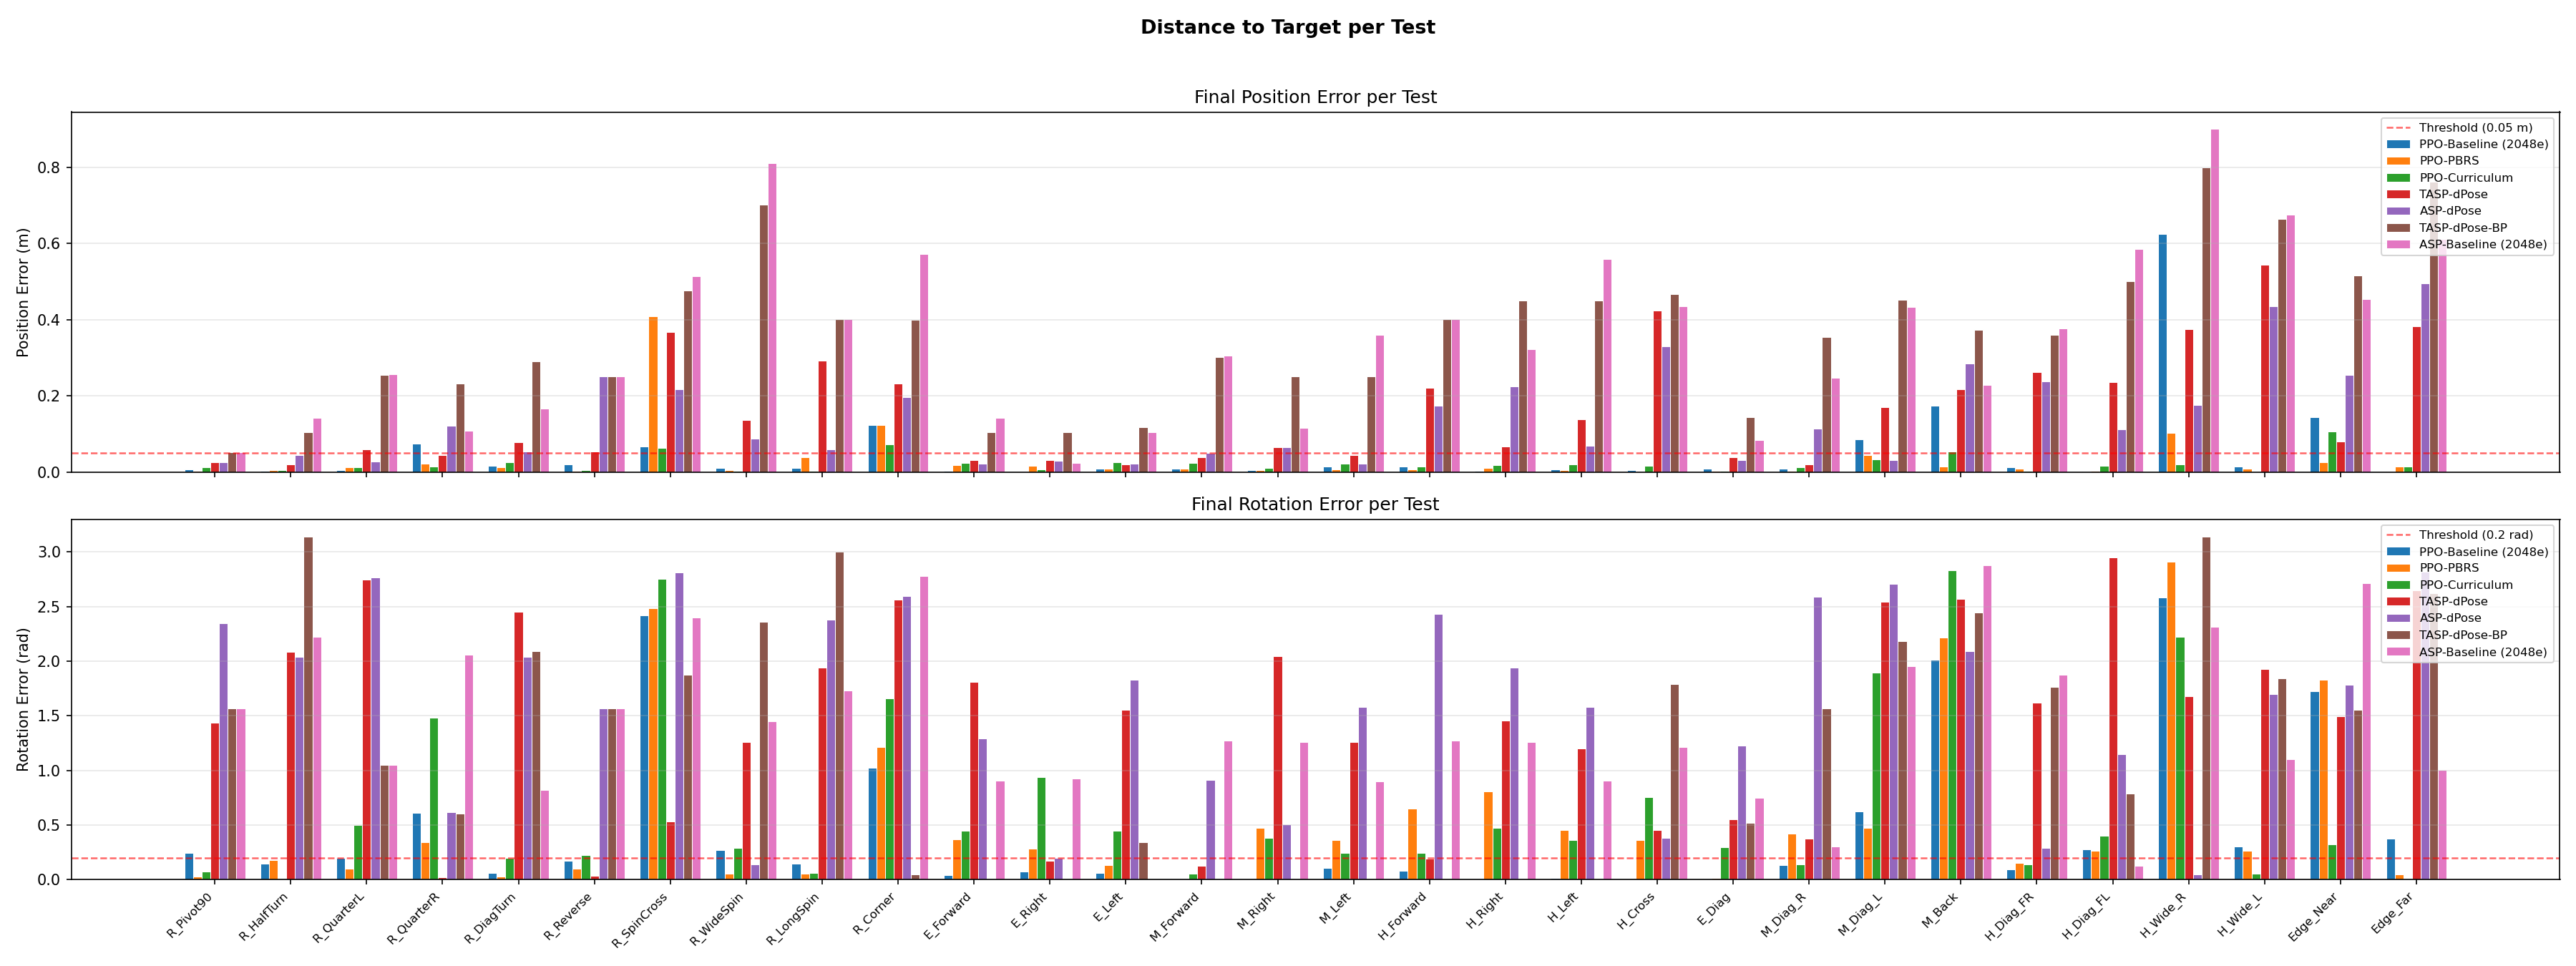
\includegraphics[width=0.85\textwidth]{figures/val_multi_error_bars.png}

  \vspace{6pt}
  {\small
  \textbf{Top:} PPO-PBRS (blue) vs PPO-Curriculum (orange) head-to-head — per-scene trial-level SR from 20 trials. Overlapping CIs on most scenes.\\
  \textbf{Bottom:} All 4 models — the self-play variants are near-zero on all but the easiest scenes.\\
  \textbf{Green labels:} position-only tests. \textbf{Purple labels:} position+rotation tests.
  }

  \vfill\litfooter{[Schulman et al.\ 2017]~[Ng et al.\ 1999]~[Grze\'s 2017]}
\end{frame}


% ============================================================
% APPENDIX: WEAKNESSES & PROTOCOL DETAILS
% ============================================================

\begin{frame}[t]{Appendix H — P82 Curriculum Trigger Bug}
  \small
  \textbf{The original PPO-Curriculum trigger never activated because it gated on an unreachable metric.}

  \vspace{4pt}
  \textbf{Broken trigger (original):}
  \[
  \text{If } \operatorname{mean}(\textit{per-push PosErr}) < 0.08\text{ m for ALL 50 consecutive iterations}
  \Rightarrow \text{activate Phase 2}
  \]

  \textbf{Why unreachable:}
  \begin{itemize}
    \item Per-push PosErr is measured after \emph{every} push, including early ones far from a freshly randomized goal (0.1--0.45 m away)
    \item The iteration-mean has a structural floor well above 0.08 m — even the \emph{best} model's validation PosErr is 0.202 m
    \item 50-iteration AND gate: one noisy iteration resets the streak
  \end{itemize}

  \textbf{Consequence:} $w_{\text{rot}} = 0.0$ permanently — rotation received zero reward signal. Model B (the pre-P82 version) was effectively position-only PPO.

  \textbf{Fix (P82):} gate on \textit{episodic position-only SR $\ge$ 0.5} over a 20-iteration lookback. This is a ``position is solved'' signal, not a per-push mean. Curriculum now activates.

  \vfill\litfooter{[See \textsection 3.1 of thesis]}
\end{frame}


\begin{frame}[t]{Appendix I — BobPenalty Fail-Fast Equilibrium}
  \small
  \textbf{Model I (TASP-dPose-BobPenalty)} adds a Bob time penalty $R_B \mathrel{+}= -\gamma_{sp}\!\cdot\!t_B$ on \emph{all} phase ends, including catastrophes.

  \vspace{4pt}
  \textbf{Why it creates a degenerate equilibrium:}
  \begin{center}
  \begin{tabular}{lccc}
    \toprule
    \textbf{Trajectory} & \textbf{PBRS + Sparse} & \textbf{Penalty ($0.5\times t_B$)} & \textbf{Total return} \\
    \midrule
    Fail on push 1  & $-10.5$ & $-0.5$ & $\mathbf{-11.0}$ \\
    Fail on push 10 & $-15.0$ & $-5.0$ & $\mathbf{-20.0}$ \\
    Succeed push 5  & $+10.0$ & $-2.5$ & $\mathbf{+7.5}$ \\
    \bottomrule
  \end{tabular}
  \end{center}

  \textbf{Mechanism:}
  \begin{enumerate}
    \item PPO's gradient pushes Bob toward higher returns — ``fail on push 1'' ($-11.0$) beats ``try for 10 pushes and fail'' ($-20.0$)
    \item Since failing is easier than succeeding in contact-rich physics, the policy collapses to immediate failure
    \item Alice's reward collapses simultaneously: $R_A = 0.5\!\cdot\!\max(0, 1-5) = 0$ — she gets zero signal
  \end{enumerate}

  \textbf{Lesson:} asymmetric reward structure (Alice incentivised, Bob unpenalised) is necessary. This is a \emph{reward design failure}, not a refutation of Sukhbaatar 2018 or Letcher 2019.

  \vfill\litfooter{[See thesis \textsection 5.4 for full diagnostic]}
\end{frame}


\begin{frame}[t]{Appendix J — Confounded Ablation Disaggregation}
  \small
  \textbf{Self-play variants differ from single-agent PPO-PBRS on $\ge$7 axes simultaneously:}

  \vspace{4pt}
  {\footnotesize
  \begin{tabular}{lcc}
    \toprule
    \textbf{Variable} & \textbf{PPO-PBRS (80.0\%)} & \textbf{Self-play (6.7--16.7\%)} \\
    \midrule
    Agent count     & 1 & 2 (Alice + Bob) \\
    Goal distribution & Fixed random & Adversarial, shifting \\
    GoalEncoder     & None & $\phi$-MLP 8D latent \\
    ABC buffer      & None & Yes (ASP-dPose) / No (TASP-dPose) \\
    Historical pool & None & Yes \\
    Episode budget  & 15 pushes/agent & 5 (Alice) $+$ 10 (Bob) \\
    PPO updates/iter& 1 & 2 (Alice, then Bob) \\
    \bottomrule
  \end{tabular}
  }

  \vspace{4pt}
  \textbf{Implication:} the 4.8$\times$ SR gap cannot be attributed to any single lever.
  \begin{itemize}
    \item TASP-dPose vs ASP-dPose isolates Alice's reward type — TASP-dPose gains $+$10pp
    \item But this is a single 1-axis experiment within a 7-axis package change
    \item We present ``self-play as implemented,'' not ``the curriculum mechanism in isolation''
  \end{itemize}

  \vfill\litfooter{[See thesis \textsection 6.3 for disaggregation analysis]}
\end{frame}


\begin{frame}[t]{Appendix K — Training Budget Comparison}
  \small
  \textbf{All PBRS variants used identical budgets. The PPO-Baseline used more compute for a direct architectural comparison.}

  \vspace{4pt}
  \begin{center}
  \begin{tabular}{lccc}
    \toprule
    \textbf{Model} & \textbf{Envs} & \textbf{Max Iter} & \textbf{Est.\ Push-Macros} \\
    \midrule
    PPO-Baseline (Fractional) & 2{,}048 & 100{,}000 & $\sim$3.07B \\
    PPO-PBRS & 528 & 3{,}000 & $\sim$23.8M \\
    PPO-Curriculum & 528 & 3{,}000 & $\sim$23.8M \\
    ASP-dPose & 528 & 3{,}000 & $\sim$23.8M \\
    TASP-dPose & 528 & 3{,}000 & $\sim$23.8M \\
    TASP-dPose-BP & 528 & 3{,}000 & $\sim$23.8M \\
    \bottomrule
  \end{tabular}
  \end{center}

  \vspace{4pt}
  \textbf{Caveats:}
  \begin{itemize}
    \item PPO-Baseline at 2,048 envs received $\sim$129$\times$ more push-macros than PBRS models
    \item Both converge to 80\% validation SR — PBRS achieves this with 4$\times$ fewer parallel envs and a fraction of the total push budget
    \item The max\_iter values are SLURM caps; actual training stopped earlier (fractional: 1,030 iters; PBRS: 2,831 iters)
  \end{itemize}

  \vfill\litfooter{[See thesis \textsection 4.2 for training configuration details]}
\end{frame}


\begin{frame}[t]{Appendix L — Validation Protocol}
  \small
  \textbf{All models evaluated under an identical protocol:}

  \vspace{4pt}
  \begin{itemize}
    \item \textbf{Scene set:} 30 held-out T-block scenes — 10 rotation-dominant (R\_*), 10 position-only (E\_*/M\_*/H\_*), 10 combined position+rotation
    \item \textbf{Trials:} 20 independent trials per scene (best-of-20); a scene is ``solved'' if \emph{any} trial meets the gate
    \item \textbf{Success gate:} $\text{pos\_err} < 0.05$ m \textbf{and} $\text{rot\_err} < 0.2$ rad at trial termination
    \item \textbf{Push budget:} up to 30 pushes per trial (training uses 5--15)
    \item \textbf{Scene SR vs Trial SR:} scene SR counts scenes where $\ge$1/20 trials pass; trial SR counts individual trial success rate
  \end{itemize}

  \vspace{4pt}
  \textbf{Disclosed limitations:}
  \begin{itemize}
    \item \textbf{Single-seed validation:} each model evaluated once (one seed per checkpoint). Training SR variance exists across 5 chains (PPO-PBRS BestSR 0.081--0.110) but validation CIs are single-model.
    \item \textbf{Protocol consistency:} some ASP variants used trial\_count=10 in early validations; later re-evaluated at trial\_count=20. The deck reports only the trial\_count=20 results.
    \item \textbf{Best-of-20 inflates scene SR:} PPO-PBRS trial SR is 66.0\% but scene SR is 80.0\% — a scene passes if \emph{any} trial succeeds.
  \end{itemize}

  \vfill\litfooter{[Full validation scripts in \texttt{asyncDualPlayPPO/tests/}]}
\end{frame}

\end{document}
